\ifdefined\isphone
  \documentclass[a6paper,11pt,oneside]{book}

\usepackage{algpseudocode}
\usepackage{algorithm}
\usepackage{amsfonts}
\usepackage{amsmath,amsthm,amssymb}
\usepackage{graphicx}
\usepackage{hyperref}
\usepackage{mathtools}
\usepackage{steinmetz}
\usepackage{fancyvrb}
\usepackage{textcomp}
\usepackage{gensymb}
\usepackage[normalem]{ulem}
\usepackage[T1]{fontenc}
\usepackage{cmap}
\usepackage{xspace}

\DeclareGraphicsExtensions{.pdf,.png,.jpg}

\newcommand{\mb}[1]{\ensuremath{\mathbb{{#1}}}}
\newcommand{\setof}[1]{\ensuremath{\left \{ #1 \right \}}}
\newcommand{\tuple}[1]{\ensuremath{\left \langle #1 \right \rangle }}

\DeclarePairedDelimiter{\ceil}{\lceil}{\rceil}
\DeclarePairedDelimiter{\floor}{\lfloor}{\rfloor}

\DeclareSymbolFont{bbold}{U}{bbold}{m}{n}
\DeclareSymbolFontAlphabet{\mathbbold}{bbold}

\newtheorem{statement}{Statement}
\newtheorem{rmk}{Remark}
\newtheorem{defi}{Definition}
\newtheorem{example}{Example}
\newtheorem{theorem}{Theorem}
\newtheorem{lemma}[theorem]{Lemma}
\newtheorem{proposition}[theorem]{Proposition}
\newtheorem{pf}[theorem]{Proof}
\newtheorem{corollary}[theorem]{Corollary}

% Differences
\usepackage[margin=5mm]{geometry}
\usepackage{tgheros}
\renewcommand*\familydefault{\sfdefault}

\else
  \documentclass[11pt,oneside]{book}

\usepackage{algpseudocode}
\usepackage{algorithm}
\usepackage{amsfonts}
\usepackage{amsmath,amsthm,amssymb}
\usepackage{graphicx}
\usepackage{hyperref}
\usepackage{mathtools}
\usepackage{steinmetz}
\usepackage{fancyvrb}
\usepackage{textcomp}
\usepackage{gensymb}
\usepackage[normalem]{ulem}
\usepackage[T1]{fontenc}
\usepackage{cmap}
\usepackage{xspace}

\DeclareGraphicsExtensions{.pdf,.png,.jpg}

\newcommand{\mb}[1]{\ensuremath{\mathbb{{#1}}}}
\newcommand{\setof}[1]{\ensuremath{\left \{ #1 \right \}}}
\newcommand{\tuple}[1]{\ensuremath{\left \langle #1 \right \rangle }}

\DeclarePairedDelimiter{\ceil}{\lceil}{\rceil}
\DeclarePairedDelimiter{\floor}{\lfloor}{\rfloor}

\DeclareSymbolFont{bbold}{U}{bbold}{m}{n}
\DeclareSymbolFontAlphabet{\mathbbold}{bbold}

\newtheorem{statement}{Statement}
\newtheorem{rmk}{Remark}
\newtheorem{defi}{Definition}
\newtheorem{example}{Example}
\newtheorem{theorem}{Theorem}
\newtheorem{lemma}[theorem]{Lemma}
\newtheorem{proposition}[theorem]{Proposition}
\newtheorem{pf}[theorem]{Proof}
\newtheorem{corollary}[theorem]{Corollary}

% Differences
\setlength{\textheight}{9.5in}
\setlength{\textwidth}{7.0in}
\setlength{\topmargin}{-0.75in}
\setlength{\oddsidemargin}{-0.25in}
\setlength{\evensidemargin}{0.75in}
\setlength{\parskip}{0.15in}
\setlength{\parindent}{0in}

\fi

\usepackage{listings}

\usepackage{color}
% Bootstrap colourings?
\definecolor{shadecolor}{rgb}{1, .580392157, .580392157}

\usepackage{fancybox}
\usepackage{calc}
\usepackage{framed}

\newcommand{\uC}{$\mu$C++}

% Allows multiline table cells.
\newcommand{\specialcell}[2][c]{%
  \begin{tabular}[#1]{@{}c@{}}#2\end{tabular}}

% Lstlisting colorings
\definecolor{pblue}{rgb}{0.13,0.13,1}
\definecolor{pgreen}{rgb}{0,0.5,0}
\definecolor{pred}{rgb}{0.9,0,0}
\definecolor{pgrey}{rgb}{0.46,0.45,0.48}

% Set the default pseudocode language:
\lstset{language=C++,
  showspaces=false,
  showtabs=false,
  breaklines=true,
  showstringspaces=false,
  breakatwhitespace=true,
  commentstyle=\color{pgreen},
  keywordstyle=\color{pblue},
  stringstyle=\color{pred},
  basicstyle=\ttfamily,
  moredelim=[il][\textcolor{pgrey}]{\$\$},
  moredelim=[is][\textcolor{pgrey}]{\%\%}{\%\%}
}

% Course Name
\title{CS 343}

% Fill in your name.
\author{Shale Craig}

% Now we will begin writing the document.
\begin{document}
    \maketitle

    % Next, we need to make a Table of Contents, List of Figures and
    % List of Tables.  You will most likely need to run LaTeX twice to
    % get these correct.  The first pass for LaTeX to figure out the
    % labels, and the second pass to put in the right references.
    \tableofcontents

    %%%%%%%%%%%%%%%%%%%%%%%%%%%%%%%%%%%%%%%%%%%%%%%%%%%%%%%%%%%%%%%%%%%%%
    %% REPORT BODY
    %%%%%%%%%%%%%%%%%%%%%%%%%%%%%%%%%%%%%%%%%%%%%%%%%%%%%%%%%%%%%%%%%%%%%
    %% \main will make the \section commands numbered again,
    %% it will also use arabic page numbers.
    \mainmatter

    \chapter{Control Flow} % (fold)
    \label{cha:control_flow}
        \begin{description}
            \item[Control Flow] is the order or flow in which individual statements are executed evaluated in a program.
            \item[Multi-Exit Loops] have at least one \verb|break| in the middle, not just in the end.
                \begin{lstlisting}
for (;;) {
    cin >> d;
    if (cin.fail()) break;
    ...
}
                \end{lstlisting}
            \item[Flag Variables] are used to explicitly implement control flow.
                \begin{lstlisting}
bool flag1 = false;
while (!flag1) {
    cin >> d;
    if (cin.fail()) flag1 = true;
    else {
        ...
    }
}
                \end{lstlisting}
                They are the variable equivalent to a \verb|goto|, since they can be set, reset, and tested at arbitrary locations in a program.
            \item[Static Multi-Level Exit] occurs when the program exits (\verb|return|s or \verb|goto|s) at multiple levels which are known exit points are known at compile-time.
                \begin{lstlisting}
L1 : {
    C1
    L2: switch ( ... ) {
        L3: while (true) {
            ... break L1;
            ... break L2;
            ... break L3;
        }
    }
}
                \end{lstlisting}
                We can use multi-level exit to remove flag variables and to remove duplicate code.
            \item[goto] goes to a line.

                Only use goto to perform static multi-level exit (i.e. to simulate a labeled break and continue).
        \end{description}
    % chapter control_flow (end)
    \chapter{Exceptions} % (fold)
    \label{cha:exceptions}
        \section{Dynamic Multi-Level Exit} % (fold)
        \label{sec:dynamic_multi_level_exit}
            We can extract code to create new methods (called \emph{modularization}), but this doesn't work with labels since labels have only routine scope.
            \begin{lstlisting}
// To illustrate the note, this will not compile.
void rtn ( ... ) {
    B2: for ( ... ) {
        if ( ... ) break B1;
    }
}
B1: for ( ... ) {
    rtn ( ... );
}
            \end{lstlisting}
            \begin{description}
                \item[Dynamic Multi-Level Exit] allows us to extend call and return semantics to go in the \emph{reverse} direction, so given $A$ calls $B$ calls $C$, we \emph{can} transfer from $C$ back to $A$, skipping $B$.
                \item[Non-Local Transfer] allows a routine to return from $C$, skip $B$ and go directly to $A$.
                It's a generalization of the \emph{multi-exit loop} and \emph{multi-level exit}.
                We can accomplish this using a \emph{label variable}.
                \begin{lstlisting}
label L;
void a (int i) {
    if ( ... ) goto L;
}
void b (int i ) {
    // L1 is a label.
    L1: L = L1;
}
void c (int i ) {
    // L2 is a label.
    L2: L = L1;
}
                \end{lstlisting}
                We go directly to the stack position that corresponds to the label, then change the PC to go to the label (\emph{transfer point}) in the routine.

                Since it can be set dynamically, control flow can't always be statically determined.
                Similar to \verb|goto|s, we can break the stack really easily using labels.

                In \textsc{C}, \verb|jmp_buf| declares a label variable, \verb|setjmp| initializes a label variable, and \verb|longjmp| goes to a label variable.
            \end{description}
        % section dynamic_multi_level_exit (end)

        \section{Traditional Approaches} % (fold)
        \label{sec:traditional_approaches}
            Without non-local transfer, we have a few options:
            \begin{description}
                \item[return codes] are special values returned that signal the caller to perform ``special'' control flow logic.

                    This mixes exceptions with normal return values and makes code difficult to read.
                    Additionally, it's easy to ``not expect'' these directives as output.
                \item[status flags] are values in shared global status flag being modified.

                    This can be delayed or overwritten by concurrent threads.
                \item[fix-up routines] are global or local routines called for an exception event to handle errors.

                    This increases the number of parameters, this increases the cost of each call when they're not used.
            \end{description}
        % section traditional_approaches (end)

        \section{Exception Handling} % (fold)
        \label{sec:exception_handling}
            Exceptional events are events that occur at low frequency, and are ancillary to an algorithm.

            Exception handling mechanisms (\textsc{ehm}) actively force programmers to work with exceptions, which allows programs to become more robust.
        % section exception_handling (end)

        \section{Execution Environment} % (fold)
        \label{sec:execution_environment}
            How exception handling mechanisms are implemented depends on the environment they're placed in.

            The \verb|finally| clause in Java and other languages exists to allow cleanup and deallocation code.
            This makes it hard to unwind the stack, because it sometimes needs to drop back into ``finally world'' before continuing propagating the error thrown.

            Given multiple stacks, exception handling becomes incredibly sophisticated - can exceptions be propagated between stacks?
        % section execution_environment (end)

        \section{Terminology} % (fold)
        \label{sec:terminology}
            \begin{description}
                \item[execution] is a language unit where exceptions can be raised.
                \item[execution type] is the type of an execution.
                \item[exception] is an instance of an exception type.
                \item[raise (throw)] is the operation that causes an exception.
                \item[propagation] directs control flow from a raise in the source to a handler.
                \item[propagation mechanism] is the mechanism (or rules) used to locate the handler for a thrown exception.

                    Most mechanisms give precedence to handlers most recently created in the call stack.
                \item[handler] is a nested code block responsible for handling a raised exception.
                It can handle by either returning, re-raising the same exception, or by raising a new exception.
                \item[guarded block] is a language block with associated handlers (i.e. a \verb|try-catch|-block).
                \item[unguarded block] is a language block with no associated handlers.
                \item[termination] is when control cannot return to where it was raised and the stack is unwound.
                \item[resumption] is when control flow can return to the raise point.
                \item[stack unwinding] is when all blocks on the faulting stack from the raise block to the guarded block are terminated, and destructors of objects are called.
                \item[EHM] refers to the overall Exception Handling Mechanism.
                It refers to the 4-tuple of:
                Exception Type +
                Raise +
                Propagation +
                Handlers +
                Exception Instance.
            \end{description}
        % section terminology (end)
        \section{Control Flow Types} % (fold)
        \label{sec:control_flow_types}
            Routine and exceptional control-flow can be characterized by two properties:
            \begin{itemize}
                \item Static/Dynamic call: routine/exception being called is looked up statically or dynamically
                \item Static/Dynamic return: after a routine or handler completes, it returns to its static or dynamic context (definition or caller).
            \end{itemize}
            We can tabulate this as the following:
                \begin{table}[h]
                    \label{tbl:control-flow}
                    \centering
                    \begin{tabular}{ r || c | c}
                                        & static call/raise & dynamic call/raise \\ \hline \hline
                        static return   & sequel            & termination exception \\ \hline
                        dynamic return  & routine           & routine-pointer, virtual-routine, resumption
                    \end{tabular}
                \end{table}
        % section control_flow_types (end)

        \section{Static Propagation (Sequel)} % (fold)
        \label{sec:static_propagation_sequel}
            \textbf{Sequels} are routines with no return value that code continues at the end of the block where the sequel is declared\footnote{Though relevant, a discussion with classmates came to the conclusion that  mentioned that he doesn't know of any languages that implement this feature.}.

                \begin{lstlisting}
void foo() {
    int i = 0;
    {
        sequel S1( ... ) { printf("one"); i++; }
        {
            sequel S2( ... ) { printf("two"); i++; }
        } // S2 returns to here.
        printf ("foo");
    } // S1 returns to here.
    printf ("bar")
    if (i == 0) {
        S1();
    } else if (i == 1) {
        S2();
    }
}
/*
 * prints:
 *     foo
 *     bar
 *     one
 *     bar
 *     two
 *     foo
 *     bar
 */
                \end{lstlisting}
            An advantage is that the handler is statically known, so it is super-duper efficient.
            A disadvantage is that sequels only work for monolithic programs because it must be statically nested where it is used (no re-use of ``generic'' sequels).
            This also prevents code from being separately compiled.
        % section static_propagation_sequel (end)

        \section{Dynamic Propagation} % (fold)
        \label{sec:dynamic_propagation}
            Both \textbf{termination} and \textbf{resumption} have dynamic raise; this works for separately-compiled programs, but is slower at runtime (lookup is not known statically).

            \subsection{Termination} % (fold)
            \label{sub:termination}
                Termination allows us to pass control from the start of propagation to a handler, then returns to a predefined position.

                Three different basic termination forms for \emph{non-recoverable} operations:
                \begin{enumerate}
                    \item \textbf{nonlocal} - general mechanism for block transfer on the call stack, but has a goto problem.
                    \item \textbf{terminate} - limited mechanism for block transfer on the call stack.

                        \begin{lstlisting}
label L;
void f ( ... ) {
    ...
    goto L;
}
int main() {
    L = L1;
    f (...);
L1:
S1: L = L2;
    f (...);
L2:
S2: ;
}
                        \end{lstlisting}
                    \item \textbf{retry} - combination of termination with special handler semantics
                        \begin{lstlisting}
char readfiles( char *files[], int N) {
    int i = 0, value;
    ifstream infile;
    infile.open( files[i] );
    while (true) {
        try {
            ... infile >> value ...;
        } retry (Eof) {
            i += 1;
            infile.close();
            if (i == N) goto Finished;
            ... infile.open( files[i] ) ...; // try again.
        }
    }
    : Finished;
}
                        \end{lstlisting}
                        Since this is easily simulated, it's not usually supported directly.
                \end{enumerate}

                Exception handlers can generate an arbitrary number of exceptions, and so can destructors.

                Destructors that throw errors during propagation cause the program to terminate:
                    \begin{lstlisting}
struct E {}
struct C {
    ~C() { throw E(); }
}
try {
    C x;
    throw E(); // Program terminates
} catch ( E ) { ... }
                    \end{lstlisting}
                This is generally because we cannot start the second exception without a handler to deal with the first exception, the first one is left hanging.
            % subsection termination (end)
            \subsection{Resumption} % (fold)
            \label{sub:resumption}
                In resumption, control transfers to a handler, and dynamically returned.
                    \begin{lstlisting}
_Event E {}; // uC++ exception label
void f() {
    _Resume E();
    cout << "control returns here" << endl;
}
void uMain::main() {
    try {
        f();
    } CatchResume ( E ) { cout << "handler 1" << endl; }
    try {
        f();
    } CatchResume ( E ) { cout << "handler 2" << endl; }
}
/*
 * output:
 *     handler1
 *     control returns here
 *     handler2
 *     control returns here
 */
                    \end{lstlisting}
            % subsection resumption (end)
        % section dynamic_propagation (end)

        \section{Implementation} % (fold)
        \label{sec:implementation}
            To implement termination and resumption, the raise needs to know the last guarded block with a handler for the raised exception type.
            % It's suggested to use a linked list that you can iterate through and check the exception types.
            % This way you can execute finally clauses as well.

            One approach is to associate a label variable with each exception type, re-setting the label variable whenever you enter and exit guarded blocks.
            This is millions of operations.

            For termination, it is necessary to unwind the stack due to activations that contain objects with destructors and finalizers; we linearly unwind the stack this way.

            If we assume there are very few exceptions compared to try entries and exits, we should choose to unwind the stack when implementing this for ourselves.
        % section implementation (end)

        \section{Exceptional Control-Flow} % (fold)
        \label{sec:exceptional_control_flow}
            In this section we give an example of what control flow looks like for the following snippet
                \begin{lstlisting}
{
    try {
        try {
            try {
                {
                    try {
                        throw E5();
                    } catch ( E7 ) {
                        ...
                    } catch ( E8 ) {
                        ...
                    } catch ( E9 ) {
                        ...
                    }
                }
            } catch ( E4 ) {
                ...
            } catch ( E5 ) {
                ...
            } catch ( E6 ) {
                ...
            }
        } catch ( E3 ) {
            ...
        }
    } catch ( E5 ) {
        ... resume/retry/terminate ... // where do these go?
    } catch ( E2 ) {
        ...
    }
                \end{lstlisting}
        % section exceptional_control_flow (end)
        \section{Additional Features} % (fold)
        \label{sec:additional_features}
            \subsection{Derived Exception Type} % (fold)
            \label{sub:derived_exception_type}
                \textbf{derived exception types} is a word for inherited exception types which allows us to catch exceptions with different levels of specificity.
                Exception type inheritance allows the handlers to match multiple exceptions.

                When subclassing, it is best catch an exception by reference, because the exception will be truncated otherwise.
                \begin{lstlisting}
struct B {};
struct D : public B {};
try {
    throw D();
} catch (B & e) {
    ... dynamic_cast<D>(e); ...
}
                \end{lstlisting}
            % subsection derived_exception_type (end)
            \subsection{Catch-Any} % (fold)
            \label{sub:catch_any}
                \textbf{Catch-any} is a mechanism to match anything, so we can finalize and deallocate variables.

                In java, this is a simple ``finally'' block, or mimed within an \verb|catch (Exception)| block.
            % subsection catch_any (end)
            \subsection{Exception Parameters} % (fold)
            \label{sub:exception_parameters}
                \textbf{Exception parameters} allow passing information from the raiser to a handler, usually in ivars of the exception object.
            % subsection exception_parameters (end)
            \subsection{Exception List} % (fold)
            \label{sub:exception_list}
                \textbf{Exception List} is a part of a routine's prototype that specifies about what types of exceptions can be thrown by the routine by its caller.
                This helps detect static detection of invalid exceptions, and runtime detection of where the exception can be converted into a special failure exception.
            % subsection exception_list (end)
        % section additional_features (end)
    % chapter exceptions (end)
    \chapter{Coroutine} % (fold)
    \label{cha:coroutine}
        A \textbf{Coroutine} is a routine that can suspend at some point, and be resumed from that point when control returns.
        Think of it as a routine which uses pauses to hold state, and continues from the same point.
        \begin{minipage}[t]{1\columnwidth}
            \begin{shaded}
                In exams and assignments, coroutines containing \textit{any} state usually receive zero marks.
            \end{shaded}
        \end{minipage}

        The state of a coroutine is a 3-tuple:
        \begin{description}
            \item[Execution location] which is the $PC$ starting at the beginning, and remembered at each suspend.
            \item[Execution state] which is the stack for that coroutine
            \item[Execution status] is a flag indicating if the coroutine is \verb|active|, \verb|inactive|, or \verb|terminated|.
        \end{description}
        There are two different types of coroutines:
        \begin{description}
            \item[Semi-Coroutines] have the ability to return execution to the caller, or call sub-routines.
            \item[Full-Coroutines] have the ability to pass execution to any other coroutine.
        \end{description}

        Internally, the implementation of both types of coroutines in \uC are the same, but how we use them is different.

        \section{Coroutine Structure in \uC} % (fold)
        \label{sec:coroutine_structure_in_uc}

            There is a \uC extension \verb|_Coroutine| class that looks like the following:
                \begin{lstlisting}
_Coroutine Fibonacci {
    int fn;
    void main() {
        int fn1, fn2;
        fn = 0; fn1 = fn;
        suspend();
        fn = 1; fn2 = fn1; fn1 = fn;
        suspend();
        while (true) {
            fn = fn1 + fn2;
            fn2 = fn1;
            fn1 = fn;
            suspend();
        }
    }
  public:
    int next() {
        resume();
        return fn;
    }
}
                \end{lstlisting}
            There's no execution state, and a main method that is suspended \& resumed.
            Each instance of a coroutine has its own stack.

            On initialization, \verb|main| is executed until the first \verb|suspend| call.
            Subsequent \verb|resume| calls continue from the previous \verb|suspend| call.

            We can recursive functionality of coroutines to write simple iterators.

            \subsection{Coroutine Construction} % (fold)
            \label{sub:coroutine_construction}
                The simplest way to write a coroutine is to write a standalone program, and convert it to a coroutine.

                We can convert a normal program to a coroutine by:
                \begin{itemize}
                    \item Putting processing code into the main
                    \item Converting reads and writes to suspend calls.
                    \item Use interface members and variables to transfer data to \& from the coroutine.
                \end{itemize}
            % subsection coroutine_construction (end)

            \subsection{Full-Coroutines} % (fold)
            \label{sub:full_coroutines}
                Semi-coroutines activate the member routine that activated it.
                Full-coroutines activate (and re-activate) any other coroutine.

                The method \verb|resume| activates the current coroutine (\verb|uThisCoroutine|), and \verb|suspend| activates the last \verb|resume|r.
                In other words, we can call \verb|B->resume| from the execution stack of \verb|A->resume|, and control passes to coroutine \verb|B| from \verb|A|.

                To have references from \verb|A| to \verb|B| and vice versa, we can pass in pointers, or creating a setter for the \verb|ivar| in the one instantiated first.

                When terminating a coroutine, execution control returns to its creator.
            % subsection full_coroutines (end)
        % section coroutine_structure_in_uc (end)

        \section{Coroutine Implementation} % (fold)
        \label{sec:coroutine_implementation}
            We can implement coroutines using either the callers stack (stackless), or creating a separate stack (stackful).
            Stackless coroutines can only suspend to the main coroutine.

            \subsection{Python} % (fold)
            \label{sub:python}
                Python implements the yield keyword that allows coroutines to return values, but not to pass control to other coroutines.
                It thus has no full coroutine implementation.
            % subsection python (end)
        % section coroutine_implementation (end)
    % chapter coroutine (end)

    \chapter{Concurrency} % (fold)
    \label{cha:concurrency}
        \begin{description}
            \item[Threads] schedule execution separately and independently from other threads.
            \item[Processes] are program components that have at least one thread, and has the same state information as a coroutine.
            \item[Tasks] are similar to processes, except it shares memory with other tasks.
            Tasks are sometimes called light-weight processes (LWP).
            \item[Parallel Execution] is when 2 or more operations occur simultaneously, which only occurs with multiple CPUs.
            \item[Concurrent Execution] is any situation where parallel execution appears to happen.
        \end{description}
        \section{Why Concurrency} % (fold)
        \label{sec:why_concurrency}
            By dividing work between multiple threads, we can capitalize on resources available to us to decrease the time it takes to execute our program.
        % section why_concurrency (end)
        \section{Why Concurrency is Hard} % (fold)
        \label{sec:why_concurrency_is_hard}
            People can do a small number of things concurrently, but fail at large numbers of things, and even more when they interact with each other.

            We need to be able to determine how and why to break up a problem into parts, decide how they react, and how reactions occur.

            We finally need to reason about and debug multiple execution paths that execute in a non-deterministic order.
        % section why_concurrency_is_hard (end)
        \section{Concurrent Hardware} % (fold)
        \label{sec:concurrent_hardware}
            All types of concurrency\footnote{the three types are multithreading for multiple threads, multitasking for multiple tasks, and multiprocessing for multiple processes} is trivially possible for a single processor (\textbf{uniprocessor}).
            We only need to context and switch threads on the CPU, and use pointers to share memory between tasks to have concurrent problems in uniprocessor systems.
            The bigger issue is that every computer has multiple CPUs these days.

            In \textbf{multiprocessor} systems, we can still share memory using pointers.
            In distributed systems, pointers don't point to the same things, so we're pretty much screwed in that case.
        % section concurrent_hardware (end)
        \section{Execution States} % (fold)
        \label{sec:execution_states}
            A thread can be in any of the states \{new, ready, running, blocked, halted \}, which are switched between in response to events.

            Since events are non-deterministic, basic operations (such as increment) are unsafe.
        % section execution_states (end)
        \section{Threading Model} % (fold)
        \label{sec:threading_model}
            \begin{description}
                \item[Threading Model] defines the relationship between CPUs and threads in a system.
                \item[Kernel Threads]\footnote{also known as \textbf{Virtual Processes}} are provided by the OS to manage CPUs.
                Kernel threads are scheduled across the CPUs.
            \end{description}
            Having more kernel threads than CPUs allows the OS to provide multiprocessing.
            A process may have multiple kernel threads to provide parallelism.
            User threads are a low-cost structuring mechanism.

            This relationship between user threads, kernel threads, and CPUs can be compared as the following:
            \begin{description}
                \item[Kernel Threading] 1:1:C - 1 user thread maps to 1 kernel thread
                \item[Generalized Kernel Threading] M:M:C - $M$ user threads map to $M$kernel threads \footnote{Java works this way}.
                \item[User Threading] N:1:C - $N$ user threads map to 1 kernel thread.
                \item[User Threading] N:M:C - $N$ user threads map to $M$ kernel threads\footnote{\uC works this way}.
            \end{description}
            Often, we omit the number of CPUs in our ratio.
            We can even add \textbf{nano thread}s on top of user threads, and \textbf{virtual machine}s under the OS.
            \begin{itemize}
                \item 1:1:C
            \end{itemize}
        % section threading_model (end)
        \section{Concurrent Systems} % (fold)
        \label{sec:concurrent_systems}
            Concurrent systems can be split into 3 major types:
            \begin{enumerate}
                \item Systems that attempt to discover concurrency - there is a limit to how much can be discovered.
                \item Systems that provide concurrency through implicit constructs - concurrency is built using specialized mechanisms
                \item Systems that provide concurrency through explicit constructs - concurrency is explicitly managed
            \end{enumerate}
            In fact, both of these are complementary, and can be built into the same system.
            \uC has only explict mechanisms.
            Some systems only have a single technique, but this is limited and awkward; when it comes to concurrency controls, more is better.
        % section concurrent_systems (end)
        \section{Speedup (Amdahl's Law)} % (fold)
        \label{sec:speedup}
            Program speedup can be denoted $S_c = \frac{T_1}{T_C}$, where $C$ is the number of CPUs, and $T_1$ is the time taken for sequential execution.

            \begin{align*}
                S_c &= \frac{T_1}{T_C} \\
                &= \frac{1}{(1-P) + \frac{P}{C}}
            \end{align*}
            Where $P$ is the proportion of a progam that can be made parallel, and $C$ is the degree of concurrency.

            As we take $\lim_{C \to \infty}$, we get the maximum speedup:
            \begin{align*}
                S_{max} &= \frac{1}{1-P}
            \end{align*}

            \subsection{Sample Question} % (fold)
            \label{sub:sample_question}
                This is a sample question from the W12 Midterm:

                \textbf{Question:}
                A program has 4 sequential stages, where each stage takes the following $N$ units of time to execute:
                $S_1 = 5$, $S_2 = 20$, $S_3 = 15$, $S_4 = 60$.
                Stages $S_2$ and $S_4$ are modified is increase their speed (i.e, reduce the time to execute)by $10$ and $20$ times, respectively.
                Show the steps in computing the total speedup for the program after the modification. \\

                \textbf{Solution:}
                We can calculate the speedup $S_C$ as the sequential speed $T_1$ over the concurrent speed $T_C$:
                \begin{align*}
                    S_C &= \frac{T_1}{T_C} \\
                    &= \frac{S_1 + S_2 + S_3 + S_4}{S_1 + \frac{S_2}{10} + S_3 + \frac{S_4}{20}} \\
                    &= \frac{5 + 20 + 15 + 60}{5 + 2 + 15 + 3} \\
                    &= 4
                \end{align*}
                Thus the overall speedup is by $4$ times.
            % subsection sample_question (end)
        % section speedup (end)
        \section{Thread Creation} % (fold)
        \label{sec:thread_creation}
            We need the following 3 things to adequately specify concurrency:
            \begin{enumerate}
                \item Thread creation\footnote{Thread creation is a primitive operation that cannot be made by fitting other operations together.}
                \item Synchronization between threads
                \item Communication between threads
            \end{enumerate}
            In \uC, we use \verb|_Task|s to emulate a cobegin segment.\footnote{These segments are effectively parallelism between threads.}

            The slowest path through all tasks synchronizing is called the \textbf{critical path}.
            \subsection{\uC \_Tasks} % (fold)
            \label{sub:uc__tasks}
                Tasks are threads in \uC.
                Calling the destructor causes the current thread to wait until the task completes execution.

                \begin{lstlisting}
_Task T1 {
    void main() {}
}
_Task T2 {
    void main() { int temp = 1; }
}

void uMain::main() {
    T1 *t1 = new T1; // start execution of T1 from its main.
    ...
    T2 *t2 = new T2; // start execution of T2 from its main.
    ...
    delete t1; // wait for T1 to complete
    ...
    delete t2; // wait for T2 to complete
}
                \end{lstlisting}
                This structure allows us to ``kick off'' the same \verb|_Task| multiple times with different arguments.
            % subsection uc__tasks (end)
        % section thread_creation (end)
        \section{Termination Synchronization} % (fold)
        \label{sec:termination_synchronization}
            A thread finishes when
            \begin{itemize}
                \item It completes execution
                \item It throws an error
                \item It is killed by its parent (not in \uC)
                \item The parent terminates (not in \uC)
            \end{itemize}
            We may trigger/react to termination to implement functionality.
        % section termination_synchronization (end)
        \section{Divide and Conquer} % (fold)
        \label{sec:divide_and_conquer}
            We use divide-and-conquer to take advantage of work that can be done individually then merged.
            Using divide and conquer, work done individually should look the same.

            Task creation order doesn't matter, but deletion order may, depending on the critical path through the tasks.
        % section divide_and_conquer (end)
        \section{Synchronization and Communication During Execution} % (fold)
        \label{sec:synchronization_and_communication_during_execution}
            Synchronization happens when one thread happens when one thread waits for another to execute until a certain point.
            This is useful for threads waiting to transfer information from one thread to another.

            One way to do this is using a \textbf{busy wait}, which is bad.
        % section synchronization_and_communication_during_execution (end)
        \section{Communication} % (fold)
        \label{sec:communication}
            After synchronization, threads can transfer information many ways.
            In the same memory, the information can be transfered by value or address.
            In different memories\footnote{For example, they are in a distributed system.}, transferring information by value is easiest.
        % section communication (end)
        \section{Critical Section} % (fold)
        \label{sec:critical_section}
            Threads may want to modify shared resources (such as a linked list).
            Multiple threads operating on the same object is problematic.
            While this is not a problem while operations are \textbf{atomic}, so we need to find a way to do this for our code.

            We call area inside an atomic operation the \textbf{critical section}, and the act of preventing simultaneous execution \textbf{mutual exclusion}.

            We can serialize all access, but this fails when there are many readers.
        % section critical_section (end)
        \section{Static Variables} % (fold)
        \label{sec:static_variables}
            Static variables are shared between all objects of that class, and may need mutual exclusion.

            The only exception for this is in task constructors, which are naturally mutually exclusive in \uC.
            It's highly suggested not to use static variables in a concurrent program.
        % section static_variables (end)
        \section{Mutual Exclusion} % (fold)
        \label{sec:mutual_exclusion}
            Mutual exclusion requires that all the following clauses are true.
            \begin{enumerate}
                \item Only one thread can be in a critical section at a time
                \item The underlying system guarantees all threads get some CPU time.
                \item Threads not in critical sections should not prevent threads from executing critical sections.
                \item We should always return to select a thread to enter a critical section.\footnote{I'm not sure what this is about. The terms \textbf{Liveness} and \textbf{indefinite postponement} are in this.}
                \item The number of threads allowed to enter a critical section after a given thread requests to enter it should be capped, so there is no \textbf{starvation} going on.
            \end{enumerate}
        % section mutual_exclusion_game (end)
        \section{Self-Testing Critical Section} % (fold)
        \label{sec:self_testing_critical_section}
            We can create self-testing critical sections by setting critical sections that abort if another thread is currently messing up our stuff:
                \begin{lstlisting}
void criticalSection () {
    ::CurrTid = &uThisTask();
    for (int i=1; i<100; i++) {
        if (::CurrTid != &uThisTask()) {
            uAbort("interference");
        }
    }
}
                \end{lstlisting}
        % section self_testing_critical_section (end)
        \section{Software Solutions} % (fold)
        \label{sec:software_solutions}
            Software Solutions to this problem must solve the problems presented in the list above.
            \subsection{Lock} % (fold)
            \label{sub:lock}
                Locks have a \textit{status} flag that indicates if a thread is in a critical section:
                \begin{lstlisting}
foo() {
    while (lock == CLOSED) {}
    lock = CLOSED;
    criticalSection();
    lock = OPEN;
}
                \end{lstlisting}
                \textbf{This strategy breaks rule 1.}
            % subsection lock (end)
            \subsection{Alternation} % (fold)
            \label{sub:alternation}
                The alternation strategy is one where a thread will go only if it is not the last one to progress through:
                \begin{lstlisting}
foo() {
    while (last == me) {}
    criticalSection();
    last = me;
}
                \end{lstlisting}
                \textbf{This strategy breaks rule 3.}
            % subsection alternation (end)
            \subsection{Declaration of Intent} % (fold)
            \label{sub:declaration_of_intent}
                The declaration of intent strategy is one where threads politely wait until no others want to enter.
                \begin{lstlisting}
foo() {
    me = WANT_IN;
    while (you == WANT_IN) {}
    criticalSection();
    me = DONT_WANT_IN;
}
                \end{lstlisting}
                \textbf{This strategy breaks rule 4.}
            % subsection declaration_of_intent (end)
            \subsection{Retract Intent} % (fold)
            \label{sub:retract_intent}
                The retraction of intent strategy is one where threads politely submit \& resubmit requests to execute the critical section.
                \begin{lstlisting}
foo() {
    while (true) {
        me = WANT_IN;
        if (you == DONT_WANT_IN) break;
        me = DONT_WANT_IN;
        while (you == WANT_IN) {}
    }
    criticalSection();
    me = DONT_WANT_IN;
}
                \end{lstlisting}
                \textbf{This strategy breaks rule 4.}
            % subsection retract_intent (end)
            \subsection{Prioritized Entry} % (fold)
            \label{sub:prioritized_entry}
                From subsection~\ref{sub:retract_intent}, we can add the ability to be a high priority thread:
                \begin{lstlisting}
foo() {
    if (this.priority == HIGH) {
        me = WANT_IN;
        while (you == WANT_IN) {}
    } else {
        while (true) {
            me = WANT_IN;
            if (you == DONT_WANT_IN) break;
            me = DONT_WANT_IN;
            while (you == DONT_WANT_IN) {}
        }
    }
}
                \end{lstlisting}
                \textbf{This strategy breaks rule 5.}
            % subsection prioritized_entry (end)
            \subsection{Dekker} % (fold)
            \label{sub:dekker}
                The Dekker algorithm doesn't break any rules.
                It uses a mixture of declared intention and alternation to achieve its goals:
                \begin{lstlisting}
foo() {
    while (true) {
        me = WANT_IN;
        if (you == DONT_WANT_IN) break;
        if (last == &me) {
            me = DONT_WANT_IN;
            while (last == &me) {} // wait for last == somebody else.
        }
    }
}
                \end{lstlisting}
                This strategy makes no assumptions about atomicity, and works on a machine where bits are scrambled during simultaneous assignment.
            % subsection dekker (end)
            \subsection{Peterson} % (fold)
            \label{sub:peterson}
                The Peterson algorithm doesn't break any rules.
                It uses a pointer to the last requester, and checks that no others want to go into the critical section:
                \begin{lstlisting}
foo() {
    while (true) {
        me = WANT_IN;
        last = &me;
        while (last == me && you == WANT_IN) {} //spin
        criticalSection();
        me = DONT_WANT_IN;
    }
}
                \end{lstlisting}
                While this doesn't break any rules, it assumes atomicity in assignment, and fails when bits are scrambled during simultaneous assignment.
            % subsection peterson (end)
            \subsection{$n$-Thread Prioritized Entry} % (fold)
            \label{sub:n_thread_prioritized_entry}
                In a case where $n$ threads want to enter a critical section, we modify the Peterson algorithm to use an array for priorities:
                We wait for all intents that are more important than us, then wait for all less-important coroutines to complete.
                \begin{lstlisting}
foo() {
    // step 1: wait for intents with higher priority to run:
    do {
        intents[priority] = WANT_IN;
        for (j = priority -1; j>= 0; --j) {
            if (intents[i] == WANT_IN) {
                intents[priority] = DONT_WANT_IN;
                while (intents[i] == WANT_IN) {} // spin
                break;
            }
        }
    } while (intents[priority] == DONT_WANT_IN);
    // step 2: wait for intents with lower priority to complete:
    for (j = priority+1; j<N; j++) {
        while (intents[j] == WANT_IN) {} //spin
    }
    criticalSection();
    intents[priority] = DONT_WANT_IN;
}
                \end{lstlisting}
                \textbf{This strategy breaks rule 5.}
                There are no algorithms that use only $n$ bits\footnote{No, this is not $O(n)$}, are deterministically (non-probabilistically) correct, and assume atomic assignment.
            % subsection n_thread_prioritized_entry (end)
            \subsection{$n$-Thread Bakery (Tickets)} % (fold)
            \label{sub:n_thread_bakery_tickets}
                In this implementation, we find the maximum value as ``ticket number'' in the array, and set our value to that.
                We then wait until we have the lowest ticket number in the array.
                In the case that multiple values are found in the array with the same ticket number, we also ensure we are the lowest priority with that value.
                \begin{lstlisting}
foo() {
    ticket[priority] = 0;
    int max = 0;
    for (int j = 0; j< n; j++) {
        int v = ticket[j];
        if (v != INT_MAX && max < v) max = v;
    }
    max += 1;
    ticket[priority] = max;
    for (int j = 0; j < n; j++) {
        while (ticket[j] < max || (ticket[j] == max && j < priority)) {} // spin
    }
    criticalSection();
    ticket[priority] = INT_MAX;
}
                \end{lstlisting}
                Since tickets cannot increase indefinitely, this is probabilistically correct.
                This also takes $nm$ bits ($m = 32$ for an int, for example).
            % subsection n_thread_bakery_tickets (end)
            \subsection{$N$-Thread Peterson} % (fold)
            \label{sub:n_thread_peterson}
                This modification of the Peterson algorithm uses a round-based race section to find the ``loser''.
                \begin{lstlisting}
foo() {
    for (int i = 1; i<N; i++) {
        intents[myId] == i; //current round
        turns[i] = myId; // MULTI-WAY RACE ALLCAPS
L:      for (int k=1; k<=n; k++) {
            if (k != myId && intents[k] >= i && turns[i] == myId) goto L;
        }
    }
    criticalSection();
    intents[myId] = 0;
}
                \end{lstlisting}
                There are $n-1$ rounds, and each round has a loser, which implies that $n - \text{round}$ winners are promoted.
                This can be implemented in only $2n\ceil{\lg n}$ bits, but assumes atomic assignments.
            % subsection n_thread_peterson (end)
            \subsection{Tournament (Taubenfeld-Buhr)} % (fold)
            \label{sub:tournament_taubenfeld_buhr}
                TODO: Determine how this works.
                TODO: High-Priority: Determine how this works. Explaining this strategy was on the F13 midterm and the W13 final.
            % subsection tournament_taubenfeld_buhr (end)
            \subsection{Arbiter} % (fold)
            \label{sub:arbiter}
                We can always create an \textit{arbiter} task that controls entry to the critical section.
                \begin{lstlisting}
client () {
    intent[me] = true;
    while (!serving[me]) {} //spin
    criticalSection();
    intent[me] = false;
    while (serving[me]) {} // wait for the arbiter to unblock me.
}
arbiter () {
    while (true) {
        for (; intent[i]; i = (i+1)%5) {} // busy wait
        serving[i] = true;
        while (intent[i] = true) {} // busy wait
        serving[i] = false;
    }
}
                \end{lstlisting}
                This implements mutual exclusion between the arbiter and each waiting client.
            % subsection arbiter (end)
        % section software_solutions (end)
        \section{Hardware Solutions} % (fold)
        \label{sec:hardware_solutions}
            Software solutions are limited by relying only on shared information between threads.
            Hardware solutions introduce a level below the software level, which allow us to make assumptions about execution (mainly atomicity).
            This only works on a single CPU - distributed programs don't have this hardware benefit.

            We use hardware instructions to get great operations that are able to observe values \textit{while} modifying them.
            \subsection{Test/Set Instruction} % (fold)
            \label{sub:test_set_instruction}
                The test/set instruction just does that.
                It returns the old value while setting the value to the new value:
                \begin{lstlisting}
testSet(type newValue, type* lock) {
    ret = lock;
    lock = newValue;
    return ret;
}
foo() {
    while (testSet(CLOSED, lock) == CLOSED) {}
    criticalSection();
    lock = OPEN;
}
                \end{lstlisting}
                In a multi-CPU computer, somewhere in hardware\footnote{The hardware bus, specifically} must guarantee multiple CPUs produce consistent output for this instruction.
            % subsection test_set_instruction (end)
            \subsection{Swap Instruction} % (fold)
            \label{sub:swap_instruction}
                The swap instruction performs a swap of two values:
                \begin{lstlisting}
swap(type& a, type& lock) {
    int temp;
    temp = a;
    a = lock;
    lock = temp;
}
foo() {
    dummy = CLOSED;
    do {
        swap(dummy, lock);
    } while (dummy == CLOSED);
    criticalSection();
    lock = OPEN;
}
                \end{lstlisting}
            % subsection swap_instruction (end)
            \subsection{Compare/Assign Instruction} % (fold)
            \label{sub:compare_assign_instruction}
                The compare and assign (caa) instruction does assignment only if the two values being compared are equal\footnote{Some alternate implementations use inequality instead of equality.}.
                \begin{lstlisting}
bool caa(type& value, type comp, type newValue) {
    if (value == comp) {
        val = newValue;
        return true;
    }
    return false;
}
foo() {
    while (!caa(lock, OPEN, CLOSED)) {}
    lock = OPEN;
}
                \end{lstlisting}
            % subsection compare_assign_instruction (end)
            \subsection{Mellor-Crummey and Scott (MCS)} % (fold)
            \label{sub:mellor_crummey_and_scott_mcs}
                MCS provides a service bound by linking waiting threads on a queue and servicing queue in FIFO.
                \begin{lstlisting}
struct MCS::Node {
    size_t waiting;
    Node *next;
}
MCS::acquire(Node &n) {
    Node *pred;
    n.next = NULL;
    pred = fetchStore(&last, &n); // pred = last, last = n
    if (pred != NULL) {
        n.waiting = true;
        pred->next = &n;
        while (n.waiting) {} // spin
    }
}
MCS::release(Node &n) {
    if (n.next == NULL) {
        if (caa(&last, &n, NULL)) return; // the last is NULL, so nobody is waiting.
        while (n.next == NULL) {};
    }
    n.next->waiting = false; // start the next node.
}
foo() {
    MCS::Node n;
    Lock.acquire(n);
    criticalSection();
    Lock.release(n);
}
                \end{lstlisting}
            % subsection mellor_crummey_and_scott_mcs (end)
        % section hardware_solutions (end)
    % chapter concurrency (end)
    \chapter{Lock Abstraction} % (fold)
    \label{cha:lock_abstraction}
        To build synchronization or mutual exclusion mechanisms, we build locks.
        \section{Lock Ontology} % (fold)
        \label{sec:lock_ontology}
            There are a bunch of different types of lock:

            \begin{description}
                \item[Spinning Locks] busy wait until an event occurs.
                In uniprocessor systems, this lock can explicitly terminate its time slice by calling \verb|yield|.
                In multiprocessor systems, it's better to begin \verb|yield|ing after $n$ event checks fail.
                \item[Blocking (Queueing) Locks] do not busy wait, but are unblocked by a mechanism until an event occurs.
            \end{description}
        % section lock_ontology (end)
        \section{Spin Lock} % (fold)
        \label{sec:spin_lock}
            Spin locks are implemented using busy waiting, which loops checking for an event:
            \begin{lstlisting}
while (testSet(lock) == CLOSED); // spin
            \end{lstlisting}
            This is slow, since it loops until someone else opens the lock, or until it is pre-empted (i.e. when its time-slice ends).
            We can increase efficiency by yielding after the checking fails:
            \begin{lstlisting}
while (testSet(lock) == CLOSED) uThisTask().yield();
            \end{lstlisting}
            Even better, adaptive spin-locks modify the number of times that they fail before they yield\footnote{Apparently this is usually implemented using a *shudder* \textsc{pid} controller.}.
            \subsection{Implementation} % (fold)
            \label{sub:implementation}
                \uC provides the non-yielding spin lock \verb|uSpinLock| and a yielding spin lock \verb|uLock|:
                \begin{lstlisting}
class uSpinLock {
    public:
        uSpinLock(); // initializes to open
        void acquire();
        void tryacquire();
        void release();
}
class uLock {
    public:
        uLock( unsigned int value = 1);
        void acquire();
        bool tryacquire();
        void release();
}
                \end{lstlisting}
                Starvation can theoretically occur, but it's rarely a problem.

                Since \verb|uSpinLock| is non-preemptive, no other tasks may execute on that processor once the lock is acquired\footnote{Apparently it is used extensively in the \uC kernel.}.
                The \verb|uLock| provided is non-preemptive and so can be used for both synchronization and mutual exclusion.

                The method \verb|tryacquire| makes one attempt, but does not wait.

                There is no problem with calling release extra times.
                In fact, release can be used to signal availability.
            % subsection implementation (end)
        % section spin_lock (end)
        \section{Blocking Locks} % (fold)
        \label{sec:blocking_locks}
            Blocking locks only make one check for openness before blocking.
            The releaser only needs to detect the blocked thread and transferring the lock.

            In general, all blocking locks have:
            \begin{itemize}
                \item State to facilitate lock semantics
                \item A list of blocked acquirers
                \item A spin lock to protect list access and state modification
            \end{itemize}

            \subsection{Synchronization Lock} % (fold)
            \label{sub:synchronization_lock}
                The sync lock is used solely to block tasks waiting to be synchronized, and it only has the ability to block.

                The acquiring task always blocks, and releases are lost when there is no waiting task.

                Often, these are called condition locks.

                \subsubsection{Implementation} % (fold)
                \label{ssub:implementation}
                    There are two types of synchronization locks:
                    \begin{description}
                        \item[External Locking] uses external locks to protect task lists
                        \item[Internal Locking] uses internal locks to protect task lists
                    \end{description}
                    For both implementations, we need to use a binary semaphore to modify or read the task list.

                    For external implementations, we need to acquire the right to modify the list beforehand.
                    Since we block after modifying the list, we need to release the modification right inside the acquire method:
                    \begin{lstlisting}
uSpinLock* m = ...;
foo() {
    m.acquire();
    syncLock.acquire(m);
}

acquire(uSpinLock & m) {
    // add to list
    m.release();
    // Point A
    // yield and block
}
                    \end{lstlisting}
                    This is so awkward, and can still be interrupted at point $A$.
                % subsubsection implementation (end)
                \subsubsection{uCondLock} % (fold)
                \label{ssub:ucondlock}
                    \uC provides an internal synchronization lock, \verb|uCondLock|.
                    \begin{lstlisting}
class uCondLock {
    public:
        uCondLock();

        /**
         * Returns false if there are tasks blocked on the queue and true otherwise.
         */
        bool empty();

        /**
         * Used to block a task from the queue of a condition.
         * This is a blocking call, and re-acquires its argument owner-lock before returning.
         */
        void wait(uOwnerLock &lock);

        /**
         * Used to un-block a task from the queue of a condition.
         * Tasks are blocked in FIFO order.
         */
        void signal();

        /**
         * Un-blocks all tasks.
         */
        void broadcast();
}
                    \end{lstlisting}
                % subsubsection ucondlock (end)
            % subsection synchronization_lock (end)
            \subsection{Binary Semaphore} % (fold)
            \label{sub:binary_semaphore}
                Dijkstra invented the binary semaphore as a blocking equivalent of a yielding spin-lock.

                This provides synchronization \textit{and} mutual exclusion, since it remembers state about an event.

                The man who invented this concept is dutch, and so are the names for acquire and release:
                \begin{description}
                    \item[Prolagen (P)] is the acquire method.
                        It is called prior the critical section.
                    \item[Verlagen (V)] is the release method.
                \end{description}
                Semaphores with only two states (open/closed) are called \textbf{binary semaphores}.
                \subsubsection{Implementation} % (fold)
                \label{ssub:implementation}
                    The implementation is really just a 3-tuple of:
                    \begin{itemize}
                        \item Blocking task list
                        \item \verb|cnt| indicates if event has occurred (i.e. if it is open.
                        \item A spin lock to protect the state.
                    \end{itemize}
                    \uC does not provide a binary semaphore, since all binary semaphores are really just counting semaphores that only count up to 1.
                    \begin{lstlisting}
BinSem::P() {
    lock.acquire();
    if (closed == true) {
        // add to blocked list
        // yield, block, and release lock
        lock.acquire(); // re-acquire the lock.
    }
    closed = true;
    lock.release();
}

BinSem::V() {
    lock.acquire();
    if (blocked.isEmpty()) {
        closed = false;
    } else {
        // remove from blocked list, and make it ready.
    }
    lock.release();
}
                    \end{lstlisting}
                % subsubsection implementation (end)
            % subsection binary_semaphore (end)
            \subsection{Mutex Lock} % (fold)
            \label{sub:mutex_lock}
                Restricting a lock to only performing mutual exclusion allows us to separate lock usage between synchronization and mutual exclusion while allowing us to optimize based on the singular function of the lock.

                Mutex locks are divided into two types:
                \begin{description}
                    \item[Single Acquisition] locks are ones that can only be acquired by the lock owner once (recursively).
                    \item[Multiple Acquisition] locks are ones that can be acquired by the lock any number multiple times\footnote{Apparently some implementations can be released any number of times, while some only need to be released once.}.
                \end{description}
                \subsubsection{Implementation} % (fold)
                \label{ssub:implementation}
                    The easiest implementation is just to add an owner state to a binary semaphore.
                    Some other implementations put the owner at the front of the queue, but this is messier.
                % subsubsection implementation (end)
                \subsubsection{uOwnerLock} % (fold)
                \label{ssub:uownerlock}
                    \uC provides a multiple-acquisition mutex-lock, \verb|uOwnerLock|.
                    \begin{lstlisting}
class uOwnerLock {
  public:
    uOwnerLock();

    /**
     * Returns NULL if there is no owner.
     */
    uBaseTask *owner();

    /**
     * Returns the number of times the lock has been acquired by the owner.
     */
    unsigned int times();

    /**
     * Refer to uLock.acquire();
     */
    void acquire();

    /**
     * Refer to uLock.tryacquire();
     */
    bool tryacquire();

    /**
     * Refer to uLock.release();
     */
    void release();
}
                    \end{lstlisting}
                % subsubsection uownerlock (end)
                \subsubsection{Stream Locks} % (fold)
                \label{ssub:stream_locks}
                    \uC offers a special mutex for I/O based on \verb|uOwnerLock| named \verb|osacquire| and \verb|isacquire| for output and input streams respectively.

                    The two are classes that acquire the object at the beginning of their lives (constructor), and release the object at the end of their lives (destructor).
                % subsubsection stream_locks (end)
            % subsection mutex_lock (end)
            \subsection{Counting Semaphore} % (fold)
            \label{sub:counting_semaphore}
                By changing the boolean in the binary semaphore to an integer that represents the number of remaining ``events'', we can:
                \begin{itemize}
                    \item Have critical sections that allow $n$ simultaneous tasks.
                    \item Allow $n$ tasks to execute only after a certain task has completed.
                \end{itemize}
                \subsubsection{Implementation} % (fold)
                \label{ssub:implementation}
                    We can implement thins by changing the flag into a counter and setting it to the maximum on creation.
                    Then we'd decrement on acquisition, and increment it on release:
                    \begin{lstlisting}
CntSem::P() {
    lock.acquire();
    --cnt;
    if (cnt < 0) {
        // add self to lock's blocked list
        // magically yield, block, and release lock.
        lock.acquire();
    }
    lock.release();
}
CntSem::V() {
    lock.acquire();
    ++cnt;
    if (cnt <= 0) {
        // remove task from blocked list and make ready
    }
    lock.release();
}
                    \end{lstlisting}
                % subsubsection implementation (end)
                \subsubsection{uSemaphore} % (fold)
                \label{ssub:usemaphore}
                    \uC provides a counting semaphore named \verb|uSemaphore| which offers more than just a binary semaphore:
                    \begin{lstlisting}
class uSemaphore {
  public:
    uSemaphore(unsigned int counter = 1);
    /**
     * Decrements the semaphore counter.
     * If the semaphore counter is >= 0 the caller continues, otherwise it blocks.
     */
    void P();

    /**
     * TryP returns true if the semaphore has been acquired and false otherwise (it basically is P without blocking)
     */
    bool tryP();

    /**
     * Wakes up the task blocked for the longest time if there are tasks blocked on the semaphore.
     * [times is the number of tasks woken up]
     */
    void V(unsigned int times = 1);

    /**
     * Returns the value of the semaphore counter:
     *  n<=0  means abs(n) tasks are blocked and the semaphore is locked
     *  n>0 means that there are n tasks that are allowed to acquire the semaphore, and it is unlocked.
     */
    int counter() const;

    /**
     * Returns false if there are threads blocked on the semaphore (and true otherwise).
     */
    bool empty() const;
}
                    \end{lstlisting}
                % subsubsection usemaphore (end)
            % subsection counting_semaphore (end)
            \subsection{Barrier} % (fold)
            \label{sub:barrier}
                A barrier coordinates a group of tasks performing a concurrent operation surrounded by sequential operations.
                Thus, it is only for synchronization and not mutual exclusion.

                Barriers are initialized to $n$, the number of tasks they will hold before allowing them to continue.

                Tasks call \verb|block|.
                The $n$th task will allow all tasks to continue.

                These can only be used for mutual exclusion.
                \subsubsection{uBarrier} % (fold)
                \label{ssub:ubarrier}
                    \uC barriers are thread-safe coroutines where the main can be resumed by the final task arriving at the barrier\footnote{The macro named ``\_Cormonitor'' is defined to be ``\_Mutex \_Coroutine''. Not that you'd know what a monitor is yet, see Section~\ref{sec:monitor}.}.
                    \begin{lstlisting}
_Cormonitor uBarrier {
  protected:
    void main { for (;;) { suspend(); } }
  public:
    uBarrier( unsigned int total );


    /**
     * returns the number of tasks being synchronized
     */
    unsigned int total() const;


    /**
     * returns the number of currently waiting tasks
     */
    unsigned int waiters() const;


    /**
     * resets the number of tasks synchronizing to to 'total'
     */
    void reset( unsigned int total );


    /**
     * Wait for the nth thread. The nth thread unblocks and calls the last.
     */
    virtual void block();


    /**
     * This is implicitly called by the last task to arrive to the barrier.
     */
    virtual void last() { resume (); }
}
                    \end{lstlisting}
                    We can create a barrier by inheriting \verb|uBarrier|, and redefining \verb|main| and possibly the block method.
                    We may even want to initialize main from a constructor.
                    Here's an example of us creating a barrier:
                    \begin{lstlisting}
_Cormonitor Accumulator : public uBarrier {
    int total_;
    uBaseTask* nth_;
    void main() {
        nth = &uThisTask();
        suspend();
    }
  public:
    Accumulator( int rows ) : uBarrier ( rows ), total_(0), nth_(0) {}
    void block( int subtotal ) {total += subtotal; uBarrier::block(); }
    int total() { return total_; }
    uBaseTask* nth() { return nth_; }
}

_Task Adder {
    int *row, size;
    Accumulator &acc;
    void main() {
        int subtotal = 0;
        for (unsigned int r = 0; r<size; r++) subtotal += row[r];
        acc.block(subtotal);
    }
  public:
    Adder (int row[], int size, Accumulator &acc) :
        size( size ), row( row ), acc( acc ) {}
}
                    \end{lstlisting}
                % subsubsection ubarrier (end)
            % subsection barrier (end)
        % section blocking_locks (end)
        \section{Lock Programming} % (fold)
        \label{sec:lock_programming}
            \subsection{Synchronization Locks} % (fold)
            \label{sub:synchronization_locks}
                Synchronization locks are weak, since we need to provide external mutual exclusion because they are weak.
            % subsection synchronization_locks (end)
            \subsection{Precedence Graph} % (fold)
            \label{sub:precedence_graph}
                \verb|P| and \verb|V| in conjunction with \textsc{cobegin} are as powerful as the \textsc{start} and \textsc{wait} commands.

                Given a list of statements where the result is compounded in some parts, we can use the graph to analyze which code and data depend on each other:
                \begin{verbatim}
                    S1: a := 1
                    S2: b := 1
                    S3: c := a + b
                    S4: d := 2 * a
                    S5: e := c + d
                \end{verbatim}
                By analyzing what data and code depends on each other, we can create a graph of dependencies, as seen in Figure~\ref{fig:precedence_graph}.
                \begin{figure}[h]
                    \centering
                    \label{fig:precedence_graph}
                    \caption{Sample Precedence Graph}
                    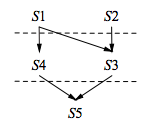
\includegraphics{images/precedence_graph.png}
                \end{figure}
                We can equivalently express this initial code using a bunch of semaphores:
                \begin{verbatim}
                    Semaphore L1(0), L2(0), L3(0), L4(0)
                    COBEGIN
                        BEGIN a:= 1; v(L1); END;
                        BEGIN b:= 2; v(L2); END;
                        BEGIN P(L1); P(L2); c :=a + b; v(L3); END;
                        BEGIN P(L1); d := 2 * a; v(L4); END;
                        BEGIN P(L3); P(L4); e := c + d; END;
                    COEND
                \end{verbatim}
                Similarly, we can create a process graph as seen in Figure~\ref{fig:process_graph}.
                \begin{figure}[h]
                    \centering
                    \label{fig:process_graph}
                    \caption{Sample Process Graph}
                    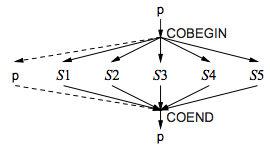
\includegraphics{images/proccess_graph.png}
                \end{figure}
            % subsection precedence_graph (end)
            \subsection{Buffering} % (fold)
            \label{sub:buffering}
                In most cases, tasks communicate in a single direction using a queue, where producers push to the queue, and consumers pop from the queue.
                \subsubsection{Unbounded Buffer} % (fold)
                \label{ssub:unbounded_buffer}
                    Two tasks will communicate through a queue of unbounded length.
                    The producer may work faster than the consumer, but this is ok since the buffer is infinite length.
                    Consumers need to wait for producers to add if they work faster than the producer.
                    \begin{lstlisting}
#define QueueSize infinity

int front = back = 0;
int Elements[QueueSize];
uSemaphore signal(0);

void Producer::main() {
    while (true) {
        // append to queue
        signal.V();
    }
    queue.append(END_SIGNAL);
}
void Consumer::main() {
    while (true) {
        signal.P();
        value = queue.pop();
        if (value == END_SIGNAL) break;
        // use the value
    }
}
                    \end{lstlisting}
                    This is an instance where a semaphore is used for synchronization.

                    The problem with unbounded buffers is that they take infinite memory\footnote{A producer moving faster than a consumer will cause the buffer to grow with respect to time. See Sub-Section~\ref{sub:buffering}.}.
                % subsubsection unbounded_buffer (end)
                \subsubsection{Bounded Buffer} % (fold)
                \label{ssub:bounded_buffer}
                    Because the queue is like bounded, producers need to wait if the buffer is full.

                    We're going to use two counting semaphores for the finite length of the shared queue:
                    \begin{lstlisting}
uSemaphore full(0), empty(QueueSize);
void Producer::main() {
    for (...) {
        item = ...
        empty.P(); // Reserve a space in the queue to append our value.
        queue.append(item);
        full.V(); // Indicate that there is a takeable item in the queue
    }
}
void Consumer::main() {
    for (...) {
        full.P(); // reserve the right to take a value
        x = queue.pop();
        empty.V(); // increase the number of values remaining
        ...
    }
}
                    \end{lstlisting}
                    This produces decent concurrency, but definitely not maximum concurrency.
                    This also allows multiple producers and multiple consumers.
                % subsubsection bounded_buffer (end)
            % subsection buffering (end)
            \subsection{Lock Techniques} % (fold)
            \label{sub:lock_techniques}
                We want to implement a split binary semaphore - a collection of semaphores which at most one has the value 1.

                We use a technique named \textbf{baton passing} which passes a (conceptual) baton\footnote{The baton is implemented as a semaphore.} between different tasks that wait on it.
                The baton is acquired in entry and exit protocol, and is passed from signaller to signalled task.
                \begin{lstlisting}
class BinSem {
    queue<Task> blocked;
    bool inUse;
    SpinLock lock;
  public:
    BinSem( bool usage = false ) : inUse( usage ) {}
    void P() {
        lock.acquire(); // Pick up baton. Now we are 'allowed' to access state.
        if ( inUse ) {
            // add self to lock's blocked list
            // yield, block and release lock at the same time

            // When unblocked:
            // We've been passed the baton. Now we can access state.
        }
        inUse = true;
        lock.release();
    }
    void V() {
        lock.acquire(); // Pick up the baton. Now we are 'allowed' to access state.
        if (!blocked.isEmpty()) {
            // remove the task from the blocked list and make it ready.
            // At this point, we've passed the baton, and cannot access state
        } else {
            inUse = false;
            lock.release();
        }
    }
}
                \end{lstlisting}
            % subsection lock_techniques (end)
            \subsection{Readers and Writer Problem} % (fold)
            \label{sub:readers_and_writer_problem}
                When there are multiple tasks that share reading and writing to a resource, we want to ensure that we are able to allow multiple concurrent readers while serializing access for writer tasks (writers may read as part of their write process).

                We're going to use split binary semaphores to segregate 3 kinds of tasks: arrivers, readers, and writers.

                \subsubsection{Solutions 1-6} % (fold)
                \label{ssub:solutions_1_6}
                    These solutions have various problems.
                    Here is an itemized list:
                    \begin{itemize}
                        \item If we allow the readers to go first, it starves the writers.
                        \item If we allow the writers to go first, it starves the readers\footnote{If it is 80\% readers and 20\% writers, course notes claim this works experimentally.}.
                        \item When tasks exit, they should activate the type that isn't their own.
                        The problem this creates is that due to the way that they can be condensed, readers that arrive after a writer may be reading stale data.
                        We should service readers and writers in \textbf{temporal order}.
                        \item When groups arrive, we should concatenate spans readers with no writers in between.
                        The textbook argues that \textit{Now we lose kind of waiting task!}.
                        % TODO: make this area more concise.
                        I'm unsure of what this means\footnote{I'd postulate that this means that we'll have more waiters, but I'm not sure.}.
                        \item If we create a ``next up'' chair... I don't really understand this one. % TODO: do section 5.4.5.5
                        \item If we create a ticked method (See Sub-Section~\ref{sub:n_thread_bakery_tickets}), we can get readers and writers to take a ticket before releasing the baton.
                        Starvation is not an issue, but this isn't efficient.
                        \item If we had a list of private semaphores... I don't really understand this one either. % TODO: do section 5.4.5.6-"Alternative"
                    \end{itemize}
                % subsubsection solutions_1_6 (end)
                \subsubsection{Solution 7} % (fold)
                \label{ssub:solution_7}
                    Generally speaking, we want a solution that provides:
                    \begin{enumerate}
                        \item Execution in temporal order
                        \item A smaller (or simpler) solution
                        \item An efficient solution
                    \end{enumerate}
                    We are going to create an ad-hoc solution that uses questionable split-binary semaphores and baton-passing.

                    Tasks wait in temporal order for an entry semaphore.
                    Writers wait on the writer chair until readers leave the resource, holding the baton until all readers leave.
                    Semaphore lock is only used for mutual exclusion.
                    \begin{lstlisting}
uSemaphore entry_q(1);
uSemaphore lock(1), writer_q(0);
void Reader::main() {
    entry_q.P(); // entry protocol.
    lock.P();
    r_cnt++;
    lock.V();
    entry_q.V(); // put the baton down
    ...
    lock.P(); // exit protocol
    r_cnt--;
    criticalSection();
    if (r_cnt == 0 && w_cnt == 1) { // if last reader and there is a writer waiting
        lock.V();
        writer_q.V(); // pass the baton.
    } else {
        lock.V();
    }
}
void Writer::main() {
    entry_q.P(); // entry protocol
    lock.P();
    if (r_cnt > 0) { // are there readers waiting?
        w++;
        lock.V();
        writer_q.P(); // wait for readers
        w_cnt--; // unblock with baton
    } else {
        lock.V();
    }
    criticalSection();
    entry_q.V();
}

                    \end{lstlisting}
                % subsubsection solution_7 (end)
            % subsection readers_and_writer_problem (end)
        % section lock_programming (end)
    % chapter lock_abstraction (end)
    \chapter{Concurrent Errors} % (fold)
    \label{cha:concurrent_errors}
        \section{Race Condition} % (fold)
        \label{sec:race_condition}
            Race conditions occur when we are missing synchronization or mutual exclusion.
            Two or more tasks race along assuming that synchronization or mutual exclusion has occurred.
            The easiest way to locate errors is through thought experiments, which are personally taxing.
        % section race_condition (end)
        \section{No Progress} % (fold)
        \label{sec:no_progress}
            \subsection{Live-Lock} % (fold)
            \label{sub:live_lock}
                Live-lock is when there is indefinite postponement.
                This is essentially caused by poor scheduling in an entry protocol.
                To fix this, there always is some mechanism to break ties on simultaneous arrival that deals effectively with live-lock.
            % subsection live_lock (end)
            \subsection{Starvation} % (fold)
            \label{sub:starvation}
                When a selection algorithm ignores $n\ge1$ tasks so they are never executed, the $n$ tasks are starved.

                While infinite starvation is very rare in real codebases, short-term starvation can occur and is problematic.

                Like a live-lock (see Sub-Section~\ref{sub:live_lock}), this includes situations where the starving task may only really switch between active, ready, and possibly blocked states.
            % subsection starvation (end)
            \subsection{Dead-Lock} % (fold)
            \label{sub:dead_lock}
                Deadlock is a state when $\ge1$ processes are waiting for an event that will never occur.
                \subsubsection{Synchronization Deadlock} % (fold)
                \label{ssub:synchronization_deadlock}
                    This occurs when $\ge1$ processes are waiting for synchronization that will never occur.
                % ssubsection synchronization_deadlock (end)
                \subsubsection{Mutual Exclusion Deadlock} % (fold)
                \label{ssub:mutual_exclusion_deadlock}
                    This occurs when processes fail to acquire resources protected by mutual exclusion.
                    There are 5 conditions for mutex-based deadlock to happen:
                    \begin{enumerate}
                        \item There exists more than 1 shared resource requiring mutual exclusion.
                        \item A process holds a resource while waiting for access to a resource held by another process (hold and wait).
                        \item Once a process has gained access to a resource, the runtime system cannot get it back (no preemption).
                        \item There exists a circular wait of processes on resources.
                        \item These conditions must occur simultaneously.
                    \end{enumerate}
                % subsubsection mutual_exclusion_deadlock (end)
            % subsection dead_lock (end)
        % section no_progress (end)
        \section{Deadlock Prevention} % (fold)
        \label{sec:deadlock_prevention}
            We want to eliminate at least one\footnote{Hopefully we can eliminate more than only one of the conditions. Doing this will increase concurrency.} of the conditions required for a deadlock from an algorithm to force deadlock to never occur.
            \subsection{Synchronization Prevention} % (fold)
            \label{sub:synchronization_prevention}
                We can eliminate all synchronization from the program to prevent synchronization-based deadlock.
                This removes communication, which means that they must generate results through side-effects (ew).
            % subsection synchronization_prevention (end)
            \subsection{Mutual Exclusion Prevention} % (fold)
            \label{sub:mutual_exclusion_prevention}
                We can eliminate deadlock by eliminating any 1 or more of the 5 conditions:
                \begin{description}
                    \item[No mutual exclusion] In many cases, it is impossible to do this while maintaining concurrency.
                    \item[No hold and wait] We can implement this by not giving any resources to a process unless all requested resources can be given.
                    This poorly utilizes resources, and introduces the possibility that we may starve a thread.
                    \item[Allow Preemption] Since preemption is dynamic, we cannot apply this statically.
                    \item[No Circular Wait] We can prevent circular wait from happening by only acquiring resources according to an ordering.
                    Threads can only acquire a resource $R_j$ if they hold no resources $R_i$ where $i \ge j$.
                    \item[Prevent Simultaneous Occurrence] We can do this by proving that the four previous rules cannot occur at the same time\footnote{There's always one dumb rule.}.
                \end{description}
            % subsection mutual_exclusion_prevention (end)
        % section deadlock_prevention (end)
        \section{Deadlock Avoidance} % (fold)
        \label{sec:deadlock_avoidance}
            Unlike deadlock prevention, deadlock avoidance monitors all blocking and allocation and detects the formation of deadlocks.
            This gives us better resource allocation at the expense of overhead.
            \begin{minipage}[t]{1\columnwidth}
                \begin{shaded}
                    % TODO: this should just be a warning, as it's not super-critical.
                    The difference between Deadlock Prevention and Deadlock Avoidance (Sections~\ref{sec:deadlock_prevention} and ~\ref{sec:deadlock_avoidance}) has been on past exams.
                \end{shaded}
            \end{minipage}
            \subsection{Banker's Algorithm} % (fold)
            \label{sub:banker_s_algorithm}
                The bankers algorithm is an iterative approach:
                We require threads $T_i$ to declare the maximum number of each type of resource that they need to complete\footnote{For example, $T_3$ needs 5 of $R_1$, 9 of $R_2$, 0 of $R_3$, and 1 of $R_4$.} execution.
                Knowing the total available resources, we check that at least one thread is able to complete to execution\footnote{We check that releasing resources allows others to complete until all threads are done.} every time we allocate a resource.

                This algorithm works, but it is limited to instances where all threads will declare how much they need prior to execution.
            % subsection banker_s_algorithm (end)
            \subsection{Allocation Graphs} % (fold)
            \label{sub:allocation_graphs}
                One way to check for potential allocation is by analyzing graphs of resource allocation, as seen in Figure~\ref{fig:allocation_graph}.
                \begin{figure}[h]
                    \centering
                    \label{fig:allocation_graph}
                    \caption{Sample Allocation Graph}
                    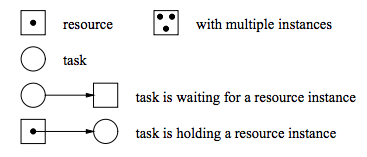
\includegraphics{images/allocation_graph.png}
                \end{figure}
                Once we have our graph, we use reductions from a complicated graph to less complicated but equivalent graphs to locate deadlocks.
                Cycles existing in our graph indicate that we have a deadlock.

                Since detecting cycles is slow, and it needs to be done at every allocation and de-allocation step, this is expensive.
            % subsection allocation_graphs (end)
        % section deadlock_avoidance (end)
        \section{Deadlock Detection and Recovery} % (fold)
        \label{sec:deadlock_detection_and_recovery}
            The idea is instead of preventing deadlocks from happening, let's just recover when they do.

            We only really have to check for a deadlock when a resource can't be allocated immediately\footnote{Checking every $t$ seconds is a second option, but I scraig postulates that a two-pronged approach is best. There is no comment about a two-pronged approach in the course notes.}.
            Recovery involves preempting\footnote{Preemption here means basically killing, restarting, or rewinding to a \textit{safe point}.} $\ge1$ processes, and restarting them at their beginning, or at a safe point.
            This isn't safe, since the victim may have made changes prior to preemption.
        % section deadlock_detection_and_recovery (end)
    % chapter concurrent_errors (end)
    \chapter{Indirect Communication} % (fold)
    \label{cha:indirect_communication}
        \verb|P| and \verb|V| are low-level primitives that protect critical sections, and establish synchronization between locks.
        This can be complicated, and can be incorrectly placed.
        Split-binary semaphores, and baton passing is hard too.
        We need higher language-level facilities that give us these things for free.
        \section{Critical Regions} % (fold)
        \label{sec:critical_regions}
            Using the pseudocode-like language which we used for \textsc{cobegin} and \textsc{coend} (see SubSection~\ref{sub:precedence_graph}):
            \begin{itemize}
                \item We can indicate shared variables (i.e. \verb|v| is protected by the \verb|MutexLock| named \verb|v_lock|:
                    \begin{verbatim}
VAR v: SHARED INTEGER MutexLock v_lock;
                    \end{verbatim}
                \item Access to shared variables is only possible from within a \textsc{region} statement:
                    \begin{verbatim}
REGION v DO                 v_lock.acquire();
    // critical section     v++; // etc
END REGION                  v_lock.release();
                    \end{verbatim}
                \item As explained in SubSection~\ref{ssub:mutual_exclusion_deadlock}, ordering these \textsc{region} calls can create deadlock.
            \end{itemize}
            This implementation prevents simultaneous reads.
            If we modified it so we can read outside the critical section, we may be reading partially updated information (ew).
        % section critical_regions (end)
        \section{Conditional Critical regions} % (fold)
        \label{sec:conditional_critical_regions}
            In our make-believe language, we're going to introduce a condition that must be true inside the mutual exclusion blocks:
            \begin{verbatim}
REGION v DO
    AWAIT conditional-expression
    ...
END REGION
            \end{verbatim}
            If \verb|conditional-expression| is false, the lock is released, and entry is re-started.
        % section conditional_critical_regions (end)
        \section{Monitor} % (fold)
        \label{sec:monitor}
            A monitor is an abstract data type that combines shared data with serializing modification.
            The key feature offered by a monitor is its differentiating set of \textbf{mutex members}\footnote{Short for mutual-exclusion member.}.
            Of the mutex members, only one may be actively executed at a time.
            Managing tasks entering and exiting from the mutex is managed automatically by the mutex.

            Basically, each monitor has a lock which is \verb|P|ed on entry to a monitor member, and \verb|V|ed on exit.
            \begin{lstlisting}
class MonitorDemo {
    MutexLock mLock;
    int v;
  public:
    int x() {
        mLock.P();
        int temp;
        try {
            ...
            temp = retVal;
            mLock.V();
        } catch(Err &e) {
            mLock.V();
            throw; // re-throw
        }
        return temp;
    }
}
            \end{lstlisting}
            Unhandled exceptions implicitly release the lock so the monitor can continue to function.
            Recursive entry is allowed\footnote{Otherwise monitors wouldn't be able to call their own methods, and recursion would be impossible without boilerplate code.}.
            Also, the destructor is blocked by a mutex, so threads can't be caught inside a monitor.
        % section monitor (end)
        \section{Scheduling (Synchronization)} % (fold)
        \label{sec:scheduling_synchronization}
            A monitor may want to schedule tasks in an order different from the order they arrive.
            \begin{description}
                \item[External Scheduling] occurs outside the monitor and is accomplished using the accept statement.
                \item[Internal Scheduling] occurs inside the monitor and is accomplished using the condition variables with signal and wait.
            \end{description}
            \subsection{External Scheduling} % (fold)
            \label{sub:external_scheduling}
                In a nutshell, accept statements block the active task on the acceptor stack and makes a task ready from the specified mutex member queue.
                Signals move a task from the specified condition to the signaled stack.

                We use the \uC \verb|_Accept| statement to control which mutex can accept calls.
                By preventing members from accepting calls at different times, we can control scheduling of tasks.
                The \verb|_Accept| statement defines what cooperation must occur for the accepting task to proceed:
                \begin{lstlisting}
_Monitor BoundedBuffer {
    int front, back, count;
    int elements[20];
  public:
    BoundedBuffer() : front(0), back(0), count(0) {}
    _Nomutex int query() { return count; }
    [_Mutex] void insert( int elem );
    [_Mutex] int remove();
};
void BoundedBuffer::insert(int elem) {
    if (coint == 20) _Accept( remove );
    elements[back] = elem;
    back = (back+1) % 20;
    count ++;
}
void BoundedBuffer::remove() {
    if (count == 0) _Accept( insert );
        // waits for insert to be called, then continues.
    int elem = elements[front];
    front = (front + 1)%20;
    count -= 1;
    return elem;
}
                \end{lstlisting}
                This implicitly queues tasks that wait outside the monitor for either \verb|insert| or \verb|remove| operations.
                Accepters block until a call to the specified mutex member occurs.
                When the accepter blocks, it is added to a stack of blocked accepters (across all methods).
                External scheduling is simple because unblocking (signalling) is implicit.
            % subsection external_scheduling (end)
            \subsection{Internal Scheduling} % (fold)
            \label{sub:internal_scheduling}
                % TODO: with permission, include a labeled diagram of stacks and queues in a mutex member.
                In a nutshell, implict scheduling occurs when a task waits in or exits from a mutex member, and a new task is selected first from the A/S\footnote{I believe that A/S is accept/signal.} stack, then the entry queue.
                Scheduling occurs for tasks inside the monitor, where \textbf{condition}s are used to create a queue of waiting tasks.
                A task waits by waiting for a \verb|uCondition x| to be true by calling \verb|x.wait()|.
                This atomically puts it at the back of the condition queue, and allows another task into the monitor by releasing the monitor lock.

                The \verb|uCondition.empty| method returns false if there are tasks blocked on the queue.
                Similarly, the \verb|uCondition.front| method returns an integer value stored with the task at the front of the condition queue.

                A task on a condition queue can be made ready by signaling the condition \verb|x.signal()|\footnote{Empty signals are lost.}.
                This readies the task, but it waits until the currently executing task is out of the monitor before continuing.
                The dual of the \verb|signal| method, \verb|x.block()| unblocks the thread and blocks the signaler.

                Generally, the entry queue is a fifo list of calling tasks to the monitor.

            % subsection internal_scheduling (end)
        % section scheduling_synchronization (end)
        \section{Readers/Writer} % (fold)
        \label{sec:readers_writer}
            See Subsection~\ref{sub:readers_and_writer_problem} to see the statement.

            We can use monitors to implement solutions to the readers/writer problem much more elegantly than if we were only using the \verb|uSemaphore| construct.
            Here is a sample of the final solution proposed, using monitors instead:
            \begin{lstlisting}
_Monitor ReadersWriter {
    int rcnt, wcnt;
  public:
    ReadersWriter() : rcnt(0), wcnt(0) {}
    void endRead() {
        --rcnt;
    }
    void endWrite() {
        wcnt = 0;
    }
    void startRead() {
        if (wcnt > 0) _Accept( endWrite );
        rcnt++;
    }
    void startWrite() {
        if (wcnt > 0) _Accept ( endWrite );
        else while ( rcnt > 0 ) _Accept( endRead );
        wcnt = 1;
    }
}
            \end{lstlisting}
        % section readers_writer (end)
        \section{Condition Signal and Wait vs Counting Semaphore P and V} % (fold)
        \label{sec:condition_signal_and_wait_vs_counting_semaphore}
            We'd like to draw the distinction between these different types:

            Calling the \verb|wait| method always blocks, while \verb|P| only blocks if the semaphore's value is less than or equal to 0.

            Calling a \verb|signal| is lost, while calling \verb|V| before \verb|P| affects the \verb|P|.

            Calling a \verb|V| may start multiple simultaneous tasks while multiple \verb|signals| only start one task at a time since they must exit serially through the monitor.

            We can simulate \verb|V| and \verb|P| through a monitor:
            \begin{lstlisting}
_Monitor semaphore {
    int sem;
    uCondition semcond;
  public:
    semaphore(int cnt = 1) : sem (cnt) {}
    void P() {
        if (sem == 0) semcond.wait();
        --sem;
    }
    void V(int incr = 1) {
        sem += incr;
        for (int i=0; i<incr; i++) semcond.signal();
    }
}
            \end{lstlisting}
        % section condition_signal_and_wait_vs_counting_semaphore (end)
        \section{Monitor Types} % (fold)
        \label{sec:monitor_types}
            Through different languages and implementations, there are subtle different ways that monitors can be implemented.
            These are usually based on their scheduling of the monitor when tasks wait, signal, and exit.

            Scheduling is the ordering of priorities for re-entering the mutex by different thread categories:
            \begin{description}
                \item[C] are the calling threads that haven't entered the mutex yet.
                \item[W] signalled (waiting) threads are the threads that were blocked then moved to a ready queue.
                \item[S] signaller threads are the ones that have signalled another thread and released control until completion\footnote{This doesn't make intuitive sense. TODO: verify.}.
            \end{description}
            To say that C < W < S means that when the mutex is choosing the next thread, it will choose the S threads before W, and before C threads.

            Monitors may either implicitly (statement) or explicitly signal (automatic signal).
            Monitors that implicitly signal may wait on condition variables or an explicit signal statement like \verb|waitUntil logicalExpression|.
            Monitors that explicitly signal call methods similar to \verb|signal|/\verb|signalWait|.

            Additionally, some monitors may be constrained to always return (leave the monitored method) as they signal.

            Refer to Table~\ref{tbl:useful-control-flow} for ten different types of control flow that are practically useful.
                \begin{table}[h]
                    \caption{Ten Different Types of Control Flow That Are Practically Useful}
                    \label{tbl:useful-control-flow}
                    \centering
                    \begin{tabular}{| c || l | l | p{3cm} | }
                        \hline
                        \textbf{Signal Type} & \textbf{Priority} & \textbf{No Priority} & \textbf{notes} \\ \hline \hline
                        Blocking & \specialcell{Priority Blocking (Hoare) \\ $C < S < W$ (\uC's signalBlock)} & \specialcell{No Priority Blocking \\ $C = S < W$} & The blocking variant requires the signaller to recheck the waiting condition in the case of a barging task. The non-blocking variant requires the signalled task to check the waiting condition in the case of a barging task. \\ \hline
                        Non-Blocking & \specialcell{Priority Non-Blocking \\ $C < W < S$ (\uC's signal)} & \specialcell{No Priority Non-Blocking \\ $C = W < S$ (Java/C\#)} & Both types have no barging (more on this later). The non-blocking variant optimizes signal before return, and the blocking variant handles internal cooperation within the monitor. \\ \hline % TODO: Where do we talk about barging?
                        Quasi-Blocking & \specialcell{Priority Quasi-Blocking \\ $C < W = S$} & \specialcell{No Priority Quasi-Blocking \\ $C = W = S$} &  This makes cooperation incredibly difficult. \\ \hline
                        Immediate Return & \specialcell{Priority Return \\ $C < W$} & \specialcell{No Priority Return \\ $C = W$} & Not powerful to handle most cases, but are simple to use in the most common case. \\ \hline
                        Implicit Signal & \specialcell{Priority Implicit Signal \\ $C < W$} & \specialcell{No Priority Implicit Signal \\ $C = W$} & Good for prototyping but poor performance. \\ \hline
                    \end{tabular}
                \end{table}
        % section monitor_types (end)
        \section{Java and C\#} % (fold)
        \label{sec:java_and_c}
            Java's concurrency constraints are descendants of Modula-3.

            \section{Threading Model} % (fold)
            \label{sec:threading_model}
                It basically defines a thread that extends a runnable:
                \begin{lstlisting}[language=Java]
    interface Thread implements Runnable {
        public Thread();
        public Thread(String name);
        public String getName();
        public void setName(String name);
        public void run();
        public synchronized void start();
        public final void join(); // waits for the thread to die
        public static Thread currentThread(); // returns the current thread
        public static void yield(); // yields the processor immediately
    }
                \end{lstlisting}
                Similarly in \uC, we have the \verb|uBaseTask| that all tasks inherit from:
                \begin{lstlisting}
    class myTask extends Thread {
        private int arg;
        private int result;
        public myTask( ... ) { ... } // task constructor
        public void run() { ... } // task main
        public void result() { return result; }
    }
                \end{lstlisting}
                Java's implementation starts threads when users call the \verb|start| method, and termination synchronization is accomplished by calling \verb|join|.
                Returning a result on thread termination is accomplished by adding member methods to the thread.
            % section threading_model (end)
            \section{The Synchronized Keyword} % (fold)
            \label{sec:the_synchronized_keyword}
                In Java, \verb|synchronized| class members help preserve mutual exclusion (should be named something along the lines of \verb|_Mutex|).
                % TODO: what does the synchronized keyword do?
            % section the_synchronized_keyword (end)


            \section{Wait, Notify, and NotifyAll} % (fold)
            \label{sec:wait_notify_and_notifyall}
                All classes have one implicit condition variable and these routines to manipulate it:
                \begin{lstlisting}
public wait();
public notify();
public notifyAll();
                \end{lstlisting}
                \subsection{Implementing a Barrier} % (fold)
                \label{sub:implementing_a_barrier}
                    Let's walk through some common pitfalls of implementing barriers (or anything) using \verb|wait|/\verb|notify|/\verb|notifyAll|.

                    \begin{lstlisting}
class Barrier {
    private int n;
    private count = 0;
    private generation = 0;
    public Barrier(int n) { this.n = n }
    public synchronized void block() {
        int mygen = generation;
        count++;
        if (count < n) {
            // We need the while loop because interrupted exceptions can cause unwanted operations.
            // Yes, a better way to do this would be to `deal with' the InterruptedException on occurance.
            while (mygen == generation)
                try {
                    wait();
                } catch (InterruptedException e) {}
        } else {
            // If we merely decrement the counter, an un-blocker that re-enters before others leave causes... bad things.
            count = 0;
            generation++;
            notifyAll();
        }
    }
}
                    \end{lstlisting}
                % subsection implementing_a_barrier (end)
                \subsection{Implementing Conditions} % (fold)
                \label{sub:implementing_conditions}
                    We can't implement \verb|_Mutex|-style conditions in Java, since that would allow us to hold the mutex while waiting for a condition to be true (that someone in tern needs access to the monitor to modify. You get the idea.).
                % subsection implementing_conditions (end)
            % section wait_notify_and_notifyall (end)
        % section java_and_c\ (end)
    % chapter indirect_communication (end)
    \chapter{Direct Communication} % (fold)
    \label{cha:direct_communication}
        While monitors work well for shared objects that therefore need mutual exclusion.
        Communication using a monitor is indirect, and clunky.

        \section{Task} % (fold)
        \label{sec:task}
            A task is like a coroutine since it has a distinguished member which has its own execution state.
            Unlike coroutines, tasks have their own thread.
            Public members of a task implicitly have the \verb|_Mutex| term; an external scheduler blocks the task's thread.

            Refer to Table~\ref{tbl:exec-properties} to see some differences between different constructs.
            \begin{table}[h]
                \caption{Execution, Member, and Object Properties}
                % TODO: should use footnotemark for these footnotes, they don't show up.
                \label{tbl:exec-properties}
                \centering
                \begin{tabular}{| l | l || r | r | }
                    \hline
                    \multicolumn{2}{|c||}{\textbf{Object Properties}} & \multicolumn{2}{|c|}{\textbf{Member Routine Properties}} \\ \hline
                    \textbf{Thread} & \textbf{Stack} & \textbf{No S/ME}\footnote{Synchronization/Mutual Exclusion} & \textbf{S/ME} \\ \hline \hline
                    No & No & class & monitor \\ \hline
                    No & Yes & coroutine  & coroutine-monitor \\ \hline
                    Yes & No & \textit{reject}\footnote{This was marked with reject in the textbook, but it doesn't have justification behind what we're rejecting. Maybe it's the concept. Maybe it's the student.} & \textit{reject} \\ \hline
                    Yes & Yes & \textit{reject?}  & coroutine-monitor \\ \hline
                \end{tabular}
            \end{table}
        % section task (end)
        \section{Scheduling} % (fold)
        \label{sec:scheduling}
            A task may want to schedule access to itself by other tasks in a non-temporal order.
            Similar to monitors, we can do this through either internal or external scheduling.

            \subsection{External Scheduling} % (fold)
            \label{sub:external_scheduling}
                Just like a monitor, tasks can use the \verb|_Accept| statement to control which mutex members of a task can accept calls.

                The when-accept setup can be expressed as the context-free-grammar:
                \begin{verbatim}
S -> T | T ELSE
T -> WHEN ACCEPT CODE | T or T
WHEN -> _When(CONDITION) | {nothing}
ACCEPT -> _Accept(METHOD)
METHOD -> [method] | METHOD, METHOD
ELSE -> _Else { ... }
                \end{verbatim}
                In the CFG, \verb|CODE| is executed after only after the \verb|_Accept| returns.

                Like a switch statement, if the accepts are conditional and false the statement does nothing.

                The optional if-like-statement \verb|_When| only allows execution of the \verb|_Accept| to progress if calls to the method exist, and the condition evaluates to true.

                If there is an \verb|_Else| clause and no \verb|_Accept| can be executed immediately, the \verb|_Else| is executed.

                \subsubsection{Accepting Order} % (fold)
                \label{ssub:accepting_order}
                    Whenever a thread accepts, this is what happens:
                    \begin{itemize}
                        \item Acceptor calls \verb|_Accept(M1)|.
                        \item Acceptor is pushed on the acceptor/signalled stack.
                        \item The accepted method is added to the acceptor/signalled stack.
                        \item Normal/implicit scheduling occurs according to C < W < S (See Section~\ref{sec:monitor_types} on monitor types/notation).
                        \item After that accept call has completed or the caller waits\footnote{I don't know of a reason. TODO: when does this happen? TODO: this doesn't make grammatical sense.}
                    \end{itemize}
                % subsubsection accepting_order (end)
            % subsection external_scheduling (end)
            \subsection{Accepting the Destructor} % (fold)
            \label{sub:accepting_the_destructor}
                To terminate tasks, we sometimes want to have a \verb|join| method.
                We could implement this as part of our main method's bajillion \verb|_Accept| statements, since it allows us to access the contents of the task after termination.

                Alternatively, we can just \verb|_Accept| on the destructor like many of our other methods:
                \begin{lstlisting}
void Foo::main() {
    while (true) {
        _Accept( ~Foo ) {
            break;
        } or ....
    }
}
                \end{lstlisting}
                The semantics for accepting a destructor aren't the same as a normal mutex member.
                When destructors are called, the caller is pushed on the acceptor/signalled stack instead of the acceptor.

                This allows it to clean up before it terminates.

                After destruction, the task behaves a monitor since threads can only enter once at a time anyways.

                Through an unspecified process, the destructor can reactiveat any blocked tasks on condition variables and/or the acceptor/signalled stack.
            % subsection accepting_the_destructor (end)
            \subsection{Internal Scheduling} % (fold)
            \label{sub:internal_scheduling}
                This is almost identical to monitor scheduling. See SubSection~\ref{sub:internal_scheduling}.
            % subsection internal_scheduling (end)
        % section scheduling (end)
        \section{Increasing Concurrency} % (fold)
        \label{sec:increasing_concurrency}
            Given that you have $\ge2$ tasks involved in direct communication\footnote{A good example is a server-client relationship.}, it is still possible to increase concurrency on both sides.
            \subsection{Server Side} % (fold)
            \label{sub:server_side}
                When using \verb|_Task|s, you have some concurrency when you're using \verb|_Accept| statements for methods.
                You have a bit more concurrency by only doing administration in the external method and doing work in the \verb|_Task| of executing the method as follows:
                \begin{lstlisting}
_Task server {
  public:
    void mem1(...) { S1.copy-in}
    voig main() {
        _Accept( mem1 ) { S1.work }
    }
}
                \end{lstlisting}
                \subsubsection{Internal Buffers} % (fold)
                \label{ssub:internal_buffers}
                    We can use internal buffers to send messages between client and server.
                    Since the size is greater than 1, clients can get in and out of the server faster.

                    The problem is that unless the average production and consumption time is the same, the buffer will always be full or empty.
                    Since the buffer is inside the task, clients still need to wait for the task to append things to it.
                    Clients that require responses are super messed as well.

                    One way is to have a worker task that aggregates and ``handles'' calls for the server.
                    The number of workers needs to balance between the number of clients to maximize concurrency throughout the application (or else we have the unbounded buffer problem).
                % subsubsection internal_buffers (end)
                \subsubsection{Administration} % (fold)
                \label{ssub:administration}
                    Administrators are servers that do nothing other than manage multiple client and worker tasks.
                    They delegate, receive, verify, route, and check work.

                    Administrators make no calls since that may block them.
                    Since they are the heart of the communication channels, this would be bad.

                    Typical worker types are:
                    \begin{description}
                        \item[timer] prompts the administrator at specified intervals
                        \item[notifier] performs a potentially blocking wait for an external event
                        \item[simple worker] performs work given to them and returns results to an administrator
                        \item[complex worker] performs work given to them and interacts directly to the of the work
                        \item[courier] performs a potentially blocking call on behalf of the administrator
                    \end{description}
                % subsubsection administration (end)
            % subsection server_side (end)
            \subsection{Client Side} % (fold)
            \label{sub:client_side}
                While servers can try to make a clients delay as short as possible, not all servers do it.

                We can overcome variable wait for the server to process a request by using asynchronous calls.
                These calls require implicit buffering between client and server to store the client's arguments from the call.
                Though \uC doesn't provide this functionality, we can (simply?) construct asynchronous from synchronous and vice versa.
                \subsubsection{Returning Values} % (fold)
                \label{ssub:returning_values}
                    If a client doesn't need results, asynchronous calls are simple.

                    When we need to return results, life isn't as simple.
                    We can divide calls into two calls:
                    \begin{lstlisting}
callee.start(args);
// do other work
x = callee.finish(); // equivalent to join.
                    \end{lstlisting}
                    The caller blocks on the finish statement for the result.
                    Depending on implementations, sometimes we need to implement a polling system where the \verb|finish| method polls the server for status until it's completed.
                % subsubsection returning_values (end)
                \subsubsection{Tickets} % (fold)
                \label{ssub:tickets}
                    Another form of protocol is a token or a ticket.

                    It calls twice:

                    \begin{itemize}
                         \item Transmits the arguments and immediately returns the ticket.
                         \item The second call passes the ticket and blocks for the result.
                     \end{itemize}
                     This can be bad if the caller doesn't retrieve the result.
                % subsubsection tickets (end)
                \subsubsection{Call-Back Routine} % (fold)
                \label{ssub:call_back_routine}
                    Callers can register a callback routine with the server task.
                    Usually, callers will release a mutex lock in the callback, and wait for it in the \verb|finish| call.

                    The advantage is that servers don't need to store the result and can drop it off immediately.
                    The other advantage is that the client can write the callback routine.

                    The disadvantage is that the client gets to write the callback routine.
                % subsubsection call_back_routine (end)
                \subsubsection{Futures} % (fold)
                \label{ssub:futures}
                    A future prevents exposing the explicit protocol on how this returning values is implemented.
                    This means that callers don't need to know how to:
                    \begin{itemize}
                        \item Poll
                        \item Handle callbacks
                    \end{itemize}
                    Futures are sub-types of the objects that they extend.

                    We can use futures as follows:
                    \begin{lstlisting}
future = callee.work(args);
...
// obtains result, blocking if necessary
i = future + ...
                    \end{lstlisting}
                    Futures are guaranteed to return empty results immediately.
                    They are lazily loaded by another thread in the future, when the result is ready.
                    Callers using the future before it is filled are blocked implicitly.

                    \uC implements two types of templated futures:
                    \begin{description}
                        \item[Explicit-Storage-Management future] (\verb|Future_ESM<T>|) must be allocated and deallocated by the client.
                        \item[Implicit-Storage-Management future] (\verb|Future_ISM<T>|) allocates and frees storage when no longer in use.
                    \end{description}
                    We focus on \verb|Future_ISM|s, since they're simpler, but less efficient.
                % subsubsection futures (end)
            % subsection client_side (end)
            \subsection{Using Futures} % (fold)
            \label{sub:using_futures}
                We can use futures on either client or server code.

                \subsubsection{Futures for Client Code} % (fold)
                \label{ssub:futures_for_client_code}
                    Here is an example of using a future for client-side stuff.
                    \begin{lstlisting}
#include <uFuture.h>
Server s;
Future_ISM f[10];
for (int i=0; i<10; i+=1)
    f[i] = server.perform(i); // start async call

...
for (int i=0; i<10; i+=1)
    osacquire(cout) << f[i] << " " << f[i]() << endl;
                    \end{lstlisting}

                    The header for \verb|Future_ISM| is as follows:
                    \begin{lstlisting}
template <typename T>
class Future_ISM/Future_ESM { // _Mutex?
  public:
    /**
     * Returns true iff the async call has completed.
     */
    bool available();

    /**
     * Returns a read-only copy of the future.
     * Blocks if the future is unavailable.
     * Raise an exception if one comes from the server.
     */
    operator()();

    /**
     * Returns a read-only copy of the future result.
     * Can only be performed if available is true
     */
    operator T();

    /**
     * Returns true iff the future is cancelled
     */
    bool cancelled();

    /**
     * Attempts to cancel the async call the future refers to.
     * Clients are unblocked and thrown a Cancellation exception is thrown.
     */
    void cancel();

    /**
     * uC++ error thrown.
     */
    _Event Cancellation{};

    /**
     * Marks the future as empty so it can be re-used.
     */
    void reset();

    /**
     * Make the result available in the future.
     * No documentation on what the return type is.
     */
    bool delivery(T result);

    /**
     * Forcibly enclose the exception into the future
     */
    bool exception(uBaseEvent *ex);
}
                    \end{lstlisting}
                % subsubsection futures_for_client_code (end)
                \subsubsection{\_Select Statement} % (fold)
                \label{ssub:_select_statement}
                    Like \verb|_Accept| statements, \verb|_Select| statements are provided to \uC for our immense benefit.

                    Essentially, they wait for some boolean combination of futures to be true.
                    \begin{lstlisting}
_Select(f1 || f2) {
    ...
}
                    \end{lstlisting}
                    The block will only be executed once either \verb|f1| or \verb|f2| has returned.
                    \begin{lstlisting}
_When(conditions) _Select (f1) {
    ...
} or _When (conditions) _Select (f2) {
    ...
}
                    \end{lstlisting}
                    We can prevent \verb|_Select| statements from being blocking using a terminating \verb|_Else| clause:
                    \begin{lstlisting}
_Select(cond1)
    ...
_When(cond2) _Else
    ...
                    \end{lstlisting}
                    As usual, \verb|_Else| clauses must be the last clause of a select statement.
                    If a \verb|_While| guard is omitted, then the \verb|_Else| clause is executed, and control continues.
                % subsubsection _select_statement (end)
            % subsection using_futures (end)
        % section increasing_concurrency (end)
        \section{Go} % (fold)
        \label{sec:go}
            Go is a cool language:
            \begin{table}[h]
                \label{tbl:go_concurrency}
                \centering
                \begin{tabular}{| r || c | c |}
                    \hline
                    Feature & Provided? & Notes \\ \hline \hline
                    Threads & Yes & goroutines are started with the go command \\ \hline
                    Synchronization & Yes & Channel with buffer size 0 \\ \hline
                    Direct Communication & Yes & Channel with buffer size 0 \\ \hline
                    Buffered communication & Yes & Channel with buffer size $n>0$ \\ \hline
                    Internal Scheduling & ??? & \\ \hline
                    External Scheduling & ??? & \\ \hline
                \end{tabular}
            \end{table}
        % section go (end)
    % chapter direct_communication (end)
    \chapter{Other Approaches to Concurrency} % (fold)
    \label{cha:other_approaches_to_concurrency}
        \section{Atomic Data Structures} % (fold)
        \label{sec:atomic_data_structures}
            Using CAA/V (See SubSection~\ref{sub:compare_assign_instruction}) to build custom things.
            We can use this to implement linked lists and queues.
            This is lock free (no locks), and is wait free (provides a bound).
        % section atomic_data_structures (end)
        \section{Coroutines} % (fold)
        \label{sec:coroutines}
            \subsection{C++ Boost} % (fold)
            \label{sub:boost}
                Provides coroutines with:
                \begin{enumerate}
                    \item Stacks
                    \item Semi and Full coroutines
                    \item No recursion
                    \item Single interface
                \end{enumerate}
                These coroutines are passed as parameters to the method (a coroutine object that you call ``yield'' on)
            % subsection boost (end)
            \subsection{Simula} % (fold)
            \label{sub:simula}
                Simula has coroutines with:
                \begin{enumerate}
                    \item Stacks
                    \item Semi and Full coroutines
                    \item Recursion
                \end{enumerate}
            % subsection simula (end)
        % section coroutines (end)
        \section{Languages With Concurrency Constructs} % (fold)
        \label{sec:languages_with_concurrency_constructs}
            \subsection{Ada 95} % (fold)
            \label{sub:ada_95}
                This language is like \uC.
                \begin{table}[h]
                    \label{tbl:ada_concurrency}
                    \centering
                    \begin{tabular}{| r || c | c |}
                        \hline
                        Feature & Provided? & Notes \\ \hline \hline
                        Threads                 & Yes & \\ \hline
                        Direct Communication    & Yes & \\ \hline
                        Buffered Communication  & Yes & \\ \hline
                        Internal Scheduling     & No & Requeue can be used to make a blocking call to another mutex member. \\ \hline
                        External Scheduling     & Yes & \\ \hline
                    \end{tabular}
                \end{table}
            % subsection ada_95 (end)
            \subsection{Concurrent C++} % (fold)
            \label{sub:concurrent_c_}
                \begin{table}[h]
                    \label{tbl:concurrent_cpp}
                    \centering
                    \begin{tabular}{| r || c | c |}
                        \hline
                        Feature                 & Provided? & Notes \\ \hline \hline
                        Threads                 & Yes & \\ \hline
                        Direct Communication    & ?? & \\ \hline
                        Buffered Communication  & No & \\ \hline
                        Internal Scheduling     & Yes & \\ \hline
                        External Scheduling     & Yes & \\ \hline
                    \end{tabular}
                \end{table}
            % subsection concurrent_c_ (end)
            \subsection{Linda} % (fold)
            \label{sub:linda}
                \begin{table}[h]
                    \label{tbl:linda}
                    \centering
                    \begin{tabular}{| r || c | c |}
                        \hline
                        Feature                 & Provided? & Notes \\ \hline \hline
                        Threads                 & Yes & \\ \hline
                        Direct Communication    & Yes & \\ \hline
                        Buffered Communication  & Yes & \\ \hline
                        Internal Scheduling     & ?? & \\ \hline
                        External Scheduling     & ?? & \\ \hline
                    \end{tabular}
                \end{table}
            % subsection linda (end)
            \subsection{Actors} % (fold)
            \label{sub:actors}
                Actors are administrators.
                \begin{table}[h]
                    \label{tbl:actors}
                    \centering
                    \begin{tabular}{| r || c | c |}
                        \hline
                        Feature                 & Provided? & Notes \\ \hline \hline
                        Threads                 & Yes & \\ \hline
                        Direct Communication    & Yes & \\ \hline
                        Buffered Communication  & Yes & \\ \hline
                        Internal Scheduling     & n/a & \\ \hline
                        External Scheduling     & n/a & \\ \hline
                    \end{tabular}
                \end{table}
                \subsubsection{Scala} % (fold)
                \label{ssub:scala}
                    \begin{table}[h]
                        \label{tbl:scala}
                        \centering
                        \begin{tabular}{| r || c | c |}
                            \hline
                            Feature                 & Provided? & Notes \\ \hline \hline
                            Threads                 & Yes & \\ \hline
                            Direct Communication    & Yes & \\ \hline
                            Buffered Communication  & Yes & Threads are tasks with a public atomic message-queue. \\ \hline
                            Internal Scheduling     & Yes & \\ \hline
                            External Scheduling     & No & \\ \hline
                        \end{tabular}
                    \end{table}
                % subsubsection scala (end)
            % subsection actors (end)
            \subsection{OpenMP} % (fold)
            \label{sub:openmp}
                Uses \verb|#pragma| to communicate concurrency to the compiler.
                \begin{table}[h]
                    \label{tbl:open_mp}
                    \centering
                    \begin{tabular}{| r || c | c |}
                        \hline
                        Feature                 & Provided? & Notes \\ \hline \hline
                        Threads                 & Yes & \\ \hline
                        Direct Communication    & Yes & \\ \hline
                        Buffered Communication  & Yes & This is a C++ extension - you can build it. \\ \hline
                        Internal Scheduling     & ??? & \\ \hline
                        External Scheduling     & ??? & \\ \hline
                    \end{tabular}
                \end{table}
            % subsection openmp (end)
        % section languages_with_concurrency_constructs (end)
        \section{Threads and Locks Library} % (fold)
        \label{sec:threads_and_locks_library}
            \subsection{Java Concurrency} % (fold)
            \label{sub:java_concurrency}
                \begin{table}[h]
                    \centering
                    \begin{tabular}{| r || c | c |}
                        \hline
                        Feature                 & Provided? & Notes \\ \hline \hline
                        Threads                 & Yes & \\ \hline
                        Direct Communication    & Yes & \\ \hline
                        Buffered Communication  & Yes & \\ \hline
                        Internal Scheduling     & Yes & \\ \hline
                        External Scheduling     & No & \\ \hline
                    \end{tabular}
                    \label{tbl:java}
                \end{table}
                scraig believes he's used concurrency in Java, so he didn't really bother taking notes for this section.
            % subsection java_concurrency (end)
            \subsection{PThreads} % (fold)
            \label{sub:pthreads}
                PThreads is to C as \uC is to C++.
                See Table~\ref{tbl:pthreads}.
                \begin{table}[h]
                    \label{tbl:pthreads}
                    \centering
                    \begin{tabular}{| r || c | c |}
                        \hline
                        Feature                 & Provided? & Notes \\ \hline \hline
                        Threads                 & Yes & \\ \hline
                        Direct Communication    & Yes & \\ \hline
                        Buffered Communication  & Self-implemented & \\ \hline
                        Internal Scheduling     & Yes & No-priority, nonblocking \\ \hline
                        External Scheduling     & Self-implemented & \\ \hline
                    \end{tabular}
                \end{table}
            % subsection pthreads (end)
            \subsection{C++11} % (fold)
            \label{sub:c_11}
                \begin{table}[h]
                    \label{tbl:cpp_11}
                    \centering
                    \begin{tabular}{| r || c | c |}
                        \hline
                        Feature                 & Provided? & Notes \\ \hline \hline
                        Threads                 & Yes & \\ \hline
                        Direct Communication    & Yes & \\ \hline
                        Buffered Communication  & Yes & \\ \hline
                        Internal Scheduling     & Yes & \\ \hline
                        External Scheduling     & Yes & \\ \hline
                    \end{tabular}
                \end{table}
            % subsection c_11 (end)
        % section threads_and_locks_library (end)
    % chapter other_approaches_to_concurrency (end)
    \chapter{Optimization} % (fold)
    \label{cha:optimization}
        We want things to be fast, because slowness is bad.
        There are three types of speedup:
        \begin{description}
            \item[Reordering] data and code is reordered
            \item[Eliding] remove unnecessary data, accesses and computation
            \item[Replication] (concurrency) allows us to duplicate stuff because of physical limitations (light, etc)
        \end{description}
        \section{Sequential Model} % (fold)
        \label{sec:sequential_model}
            Program execution is in sequential program order.

            In this model, we can reorder and elide operations that can be reordered or are unnecessary.
            We can even overlap code execution by executing concurrently (parallelism), but concurrency is limited.
        % section sequential_model (end)
        \section{Concurrent Model} % (fold)
        \label{sec:concurrent_model}
            In the concurrent model, there's everything we've talked about this term.
            Most concurrent applications are large sections of sequential code followed by small sections of concurrent code.

            Concurrent sections can be corrupted by implicit serial optimizations, so we need to identify concurrent code and restrict its optimization.
            \subsection{Disjoint Reordering} % (fold)
            \label{sub:disjoint_reordering}
                TODO: Not sure what all the $W \to R$, $W \to W$, $R \to W$ stuff is. It's in section 10.2

                There are two concurrency model terms we need to know:
                \begin{description}
                    \item[Atomically Consistent] there is an absolute ordering and a global clock.
                        In this model, every operation is ordered by real time and everyone must see the exact same ordering.
                        If A happens before B in real time, then everyone must observe that A happens before B.
                    \item[Sequentially Consistent]
                        A sequence $S$ is said to be Sequentially Consistent (SC) if there exists at least one sequential (serial) re-ordering $S'$ of tasks such that an assignment of a variable $X$ by task $T_1 \in S$ then read by task $T_2 \in S$ is the same as the value of $X$ written and read by $T_1$ and $T_2$ in $S'$.

                        In this model, there is a global ordering of writes, but no global clock of the time of the write.
                        In a sequentially consistent model, everyone must see the same ordering of writes.
                        However, this ordering does not have to match the real time ordering.
                        Even though a write A happens before a write B in real time, as long as everyone observes the same ordering (say B before A), the system is still sequentially consistent.
                        \textit{But}, writes from a single task cannot be reordered.
                \end{description}
            % subsection disjoint_reordering (end)
            \subsection{Eliding} % (fold)
            \label{sub:eliding}
                Eliding (See the beginning of Chapter~\ref{cha:optimization}) can cause errors due to copying flags to registers, and removing sleeps necessary to wait for signals\footnote{While it isn't the best thing to do, it is still valid code.}.
            % subsection eliding (end)
            \subsection{Overlapping} % (fold)
            \label{sub:overlapping}
                Implicit parallelism must synchronize before using values modified in multiple threads.
            % subsection overlapping (end)
        % section concurrent_model (end)
        \section{Corruption} % (fold)
        \label{sec:corruption}
            We make implicit assumptions about sequential execution that fails in concurrent code.
            \subsection{Memory} % (fold)
            \label{sub:memory}
                To have sequential consistency, hardware must serialize memory access and modification.

                Reads and writes can arrive in any order, and the reordering we implement support must be no different than the range a time-slice reordering provides.
                To read $A$, we need to wait for writing $A$ to complete before this happens.

                One way to do this is to buffer writes.
                CPUs wait on reads until data arrives.

                We can increase performance by disjointly reordering from $W \to R$ to $R \to W$.
                In fact, reads can bypass a buffer if the address is not waiting to write, which is bad.

                As the number of processors increase, we'd want to use more buffers, but this would allow parallel reads.

                To increase concurrency, we can eliminate serializing writes, which would allow $R \to W$ reordering from $W \to R$ and $W \to R$ reordering from $R \to W$.
                These are bad, so we can't do it.
            % subsection memory (end)
            \subsection{Cache} % (fold)
            \label{sub:cache}
                \subsection{Review} % (fold)
                \label{sub:review}
                    CPUs are fast, memory is slow.
                    The disk is the slowest.

                    We have billions of bytes, but only few registers, so we move frequently accessed data to registers.
                    When we have more data than registers, we load memory dynamically.
                    To prevent multiple threads from thrashing memory when they context switch, we use a hardware cache to stage data without pushing to memory.

                    By using multi-level caches, we get more and more size, but less speed.
                % subsection review (end)
                \subsection{Cache Coherence} % (fold)
                \label{sub:cache_coherence}
                    Caches exist for each processor, which means that values are duplicated.
                    As we move things up the hierarchy, it becomes invalid as other ones write them and needs to be invalidated.

                    \begin{description}
                        \item[Cache Coherence] is a hardware protocol ensuring duplicate values are updated
                        \item[Cache Consistency] is the name of the entire topic, and the time that caches eventually become consistent.
                    \end{description}

                    % Lazy cache consistency is something they introduce, is rarely\footnote{[TODO] Citation needed} used in practice, and doesn't allow you to always guarantee that you're reading the latest data.
                % subsection cache_coherence (end)
            % subsection cache (end)
            \subsection{Registers} % (fold)
            \label{sub:registers}
                Each processor has a bunch of registers that aren't concurrent.

                Loading a variable into a register hides its value from the main memory.
                It's impossible to peek at registers of a processor.

                The \textbf{volatile} keyword means that variables updating the main memory happens faster.
            % subsection registers (end)
            \subsection{Out of Order Execution} % (fold)
            \label{sub:out_of_order_execution}
                Cache and memory buffers will perform simple instruction reordering for reads and writes over small sections of code.

                This can mess up things like entry protocols, etc.
            % subsection out_of_order_execution (end)
        % section corruption (end)
        \section{Selectively Disabling Optimizations} % (fold)
        \label{sec:selectively_disabling_optimizations}
            We can do a few things to prevent optimizations, but most of these are compiler-specific, and diverse.

            Refer to the course notes for the list of compiler-specific modifications.
        % section selectively_disabling_optimizations (end)
    % chapter optimization (end)
\end{document}

% The majority of the final exam covers the material in the course notes from Section 6 to Section 11
